%; whizzy chapter
% -initex iniptex -latex platex -format platex -bibtex jbibtex -fmt fmt
% $B0J>e(B whizzytex $B$r;HMQ$9$k>l9g$N@_Dj!#(B


%     Tokyo Debian Meeting resources
%     Copyright (C) 2009 Junichi Uekawa

%     This program is free software; you can redistribute it and/or modify
%     it under the terms of the GNU General Public License as published by
%     the Free Software Foundation; either version 2 of the License, or
%     (at your option) any later version.

%     This program is distributed in the hope that it will be useful,
%     but WITHOUT ANY WARRANTY; without even the implied warranty of
%     MERCHANTABILITY or FITNESS FOR A PARTICULAR PURPOSE.  See the
%     GNU General Public License for more details.

%     You should have received a copy of the GNU General Public License
%     along with this program; if not, write to the Free Software
%     Foundation, Inc., 51 Franklin St, Fifth Floor, Boston, MA  02110-1301 USA

%  preview (shell-command (concat "evince " (replace-regexp-in-string "tex$" "pdf"(buffer-file-name)) "&"))
% $B2hA|%U%!%$%k$r=hM}$9$k$?$a$K$O(Bebb$B$rMxMQ$7$F(Bboundingbox$B$r:n@.!#(B
%(shell-command "cd image200903; ebb *.png")

%%$B$3$3$+$i%X%C%@3+;O!#(B

\documentclass[mingoth,a4paper]{jsarticle}
\usepackage{monthlyreport}

% $BF|IU$rDj5A$9$k!"Kh7nJQ$o$j$^$9!#(B
\newcommand{\debmtgyear}{2009}
\newcommand{\debmtgmonth}{3}
\newcommand{\debmtgdate}{21}
\newcommand{\debmtgnumber}{50}



\begin{document}

\begin{titlepage}
\thispagestyle{empty}

% $B%?%$%H%k%Z!<%8(B:$BJT=8I,MW$JItJ,$O:G=i$N%^%/%m$KHt$P$9$3$H(B

\vspace*{-2cm}
$BBh(B\debmtgnumber{}$B2s(B $BEl5~%(%j%"(B Debian $BJY6/2q;qNA(B

\hspace*{-2.4cm}
\includegraphics[width=210mm]{image200801/2008title.eps}\\
\hfill{}\debmtgyear{}$BG/(B\debmtgmonth{}$B7n(B\debmtgdate{}$BF|(B

\end{titlepage}

\dancersection{Introduction}{$B>e@n(B $B=c0l(B}

\begin{multicols}{2}
 
 
 $B:#7n$N(BDebian$BJY6/2q$X$h$&$3$=!#$3$l$+$i(BDebian$B$N@$3&$K$"$7$rF'$_F~$l$k$H(B
 $B$$$&J}$b!"$9$G$K$I$C$W$j$H$D$+$C$F$$$k$H$$$&J}$b!"7n$K0l2s(BDebian$B$K$D$$(B
 $B$F8l$j$^$;$s$+!)(B

 Debian$BJY6/2q$NL\E*$O2<5-$G$9!#(B

 \begin{itemize}
 \item \underline{Debian Developer} ($B3+H/<T(B)$B$N0i@.!#(B
 \item $BF|K\8l$G$N!V(B\underline{$B3+H/$K4X$9$k>pJs(B}$B!W$r@0M}$7$F$^$H$a!"%"%C%W%G!<%H$9$k!#(B
 \item \underline{$B>l(B}$B$NDs6!!#(B
 \begin{itemize}
  \item $BIaCJ$P$i$P$i$J>l=j$K$$$k?M!9$,(B face-to-face $B$G=P2q$($k>l$rDs6!(B
	$B$9$k!#(B
  \item Debian $B$N$?$a$K$J$k$3$H$r8l$k>l$rDs6!$9$k!#(B
  \item Debian$B$K$D$$$F8l$k>l$rDs6!$9$k!#(B
 \end{itemize}
 \end{itemize}		

 Debian$B$NJY6/2q$H$$$&$3$H$G5f6KE*$K$O;22C<TA40w$,(BDebian Package$B$r$,$j$,$j(B
 $B$H:n$k%9!<%Q!<%O%C%+!<$K$J$C$?;Q$rLQA[$7$F$$$^$9!#>pJs$N6&M-!&3hMQ$rDL$7(B
 $B$F(B Debian$B$N:#8e$NG=F0E*$JE83+$X$NEZBf$H$7$F!"!V>l!W$H$7$F$N6u4V$rDs6!$9(B
 $B$k$N$,L\E*$G$9!#(B

 2009$BG/$N7W2h$O2>$G$9!#(B

 \begin{enumerate}
  \item $B?7G/$N4k2h(B ($B%"%s%5%s%V%k2.7&3+:E(B)
  \item OSC Tokyo
  \item VAIO P $B%$%s%9%H!<%k5-O?!"(B
	$B%+!<%M%kFI=q2q!!%G%#%9%H%j%S%e!<%7%g%sBg=89g(B($B>.NS$5$s(B)($BEl5~Bg3X(B?)
  \item Git Handson ($B4d>>(B)($B$"$s$5$s$V$k2.7&(B?)
  \item $B2H(BDebian$B%5!<%P(B vs $B?&>l$N%M%C%H%o!<%/(B($B@iBeED6hETN)?^=q4[(B?\footnote{\url{http://www.library.chiyoda.tokyo.jp/}})
  \item Asterisk ($BEl5~Bg3X(B?)
  \item $B%9%Z%$%s$K$F3+:E(B
  \item Debconf$BJs9p2q(B
  \item OSC Fall?
  \item udev + HAL($B4d>>$5$s(B)
  \item 3D graphics $B3+H/!JF#Bt$5$s!K(B 
  \item Debian $B%5!<%P(B+VMware + $B3F<o(BOS$B!"(B
	$BB>$N2>A[2=%D!<%k(B(vserver etc.)$B!"(B
	$BK:G/2q(B
 \end{enumerate}

 $B2q>l8uJd$H$7$F$O2<5-$,$"$j$^$9(B:

 \begin{itemize}
  \item $BBg3X(B
  \item $B7CHf<w(BSGI$B%[!<%k(B
  \item Google$B%*%U%#%9(B
  \item $B8xL14[(B($B$"$s$5$s$V$k2.7&Ey(B)
  \item $BETN)2q5D<<(B($BL5@~(BLAN)
  \item $B7rJ]$N;\@_(B
 \end{itemize}

\end{multicols}


\newpage

\begin{minipage}[b]{0.2\hsize}
 \definecolor{titleback}{gray}{0.9}
 \colorbox{titleback}{\rotatebox{90}{\fontsize{80}{80} {\gt $B%G%S%"%sJY6/2q(B} }}
\end{minipage}
\begin{minipage}[b]{0.8\hsize}
\hrule
\vspace{2mm}
\hrule
%
% there are too many entries in 200901, usually
% we have tocdepth=2.
%
\setcounter{tocdepth}{1}
\tableofcontents
\vspace{2mm}
\hrule
\end{minipage}

\dancersection{$B:G6a$N(BDebian$B4XO"$N%_!<%F%#%s%0Js9p(B}{$B>e@n(B $B=c0l(B}
\subsection{$BEl5~%(%j%"(BDebian$BJY6/2q(B48$B2sL\Js9p(B}
% (query-replace-regexp "<.*?>" "")
% (query-replace-regexp "^[	 ]\+" "")

2009$BG/(B1$B7n(B17$BF|EZMKF|$K(B
$BEl5~%(%j%"(BDebian$BJY6/2q$N(B
$BBh(B48$B2s(B
$B$r3+:E$7$^$7$?!#(B

$B:#2s$N;22C<T$O(B
id774$B$5$s!"(B
$B$"$1$I$5$s!"(B
$BA0ED9LJ?$5$s!"(B
$B>.<<J8$5$s!"(B
$B;3K\9@G7$5$s!"(B
$B4d>>?.MN$5$s!"(B
$B$d$^$@$?$/$^$5$s!"(B
$B$8$D$+$?$5$s!"(B
$B%-%?%O%i$5$s!"(B
$B>.NS576)$5$s!"(B
$BF#BtM}Ao$5$s!"(B
$B>e@n$N(B12$BL>$G$7$?!#(B

$B%/%$%:$K$D$$$F$O!":#2s$O>.NS$5$s$,Ev=iIT:_$@$C$?$N$H(B
$B%/%$%:$rMQ0U$7$F$$$J$+$C$?$N$G%-%c%s%;%k$G$9!#(B
$B2?$+JL$N4k2h$r4|BT$7$?$$$H$3$m$G$9!#(B

$B:G=i$K:G6a$N%$%Y%s%H$N>R2p$r$7$^$7$?!#(B
$BA02s$NJY6/2q$N$*$5$i$$$H!"(B
Debian JP $B$G9T$C$?(BIAX$B2q5D$K$D$$$F>R2p$7$^$7$?!#(B
IAX$B$G$N2;@<2q5D$K6=L#$r$=$=$i$l$??M$b$$$?$h$&$G$9!#(B

\url{http://pspunch.com/pd/article/asterisk_meetme_ja.html}$B$K$F(B
$B:#2sMxMQ$7$?@_Dj$,>R2p$5$l$F$$$^$9!#(B

$B$^$::G=i$K;vA02]Bj$r>R2p$7$^$7$?!#(B

2009$BG/$K$I$&$$$&FbMF$r<B;\$9$k$N$+$K$D$$$F5DO@$7$^$7$?!#(B
$B%V%l%$%s%9%H!<%_%s%0$r$7$F$=$N$"$H(B2009$BG/$NKh7n$N7W2h$r$?$F$^$7$?!#(B
$B:#G/$OL5;v$K$G$-$k$+$J(B?

$B:G8e$KE_5Y$_$N=IBj$rH/I=$7$"$C$F=*N;!#(B

$B>e@n$O(BGit format-patch$B$rMxMQ$7$?%o!<%/%U%m!<$G$$$+$K%3%s%U%j%/%H$rH/@8(B
$B$5$;$J$$$+$r>R2p$7$^$7$?!#(B
$BA0ED$5$s$O(BMacBook$B$K(BLenny$B$r%$%s%9%H!<%k$7$J$*$7$?$H$-$K$O$^$C$?FbMF!#(B
$B>.<<$5$s$O!"(BGoogle Ajax API $B$N>R2p!#(B
id774$B$5$s$O(BAspire One $B$K%$%s%9%H!<%k$7$?$H$-$NOC!#(B
$B;3K\9@G7$5$s$O(B2ch$B%S%e!<%"!<%Q%C%1!<%8$K$D$$$F!#(B
$B4d>>$5$s$O(B Linux Kernel $B$N(B .config $B<+F0@8@.%D!<%k$K$D$$$F$N>R2p$G$7$?!#(B

\subsection{$BEl5~%(%j%"(BDebian$BJY6/2q(B49$B2sL\Js9p(B}
% (query-replace-regexp "<.*?>" "")
% (query-replace-regexp "^[	 ]\+" "")

$BBh(B49$B2sEl5~%(%j%"(BDebian$BJY6/2q$O(BOSC2009 Tokyo/Spring$B!wF|K\EE;R@lLg3X9;$K;22C$7$F$-$^$7$?!#(B

$B%;%_%J!<$H$7$F$O%O%s%:%*%s$rFsOH9T$$!"(BCDBS$B$rMQ$$$?(BDebian$B%Q%C%1!<%8:n@.$rEA<x$7$^$7$?!#(B
$B;22C<T$OA40w$G(B30$BL>6/!"EvF|Ht$SF~$j$,(B4$BL>$$$^$7$?!#(B
$B%O%s%:%*%s$r$d$C$F$_$k$H!";22C<T$N%9%-%k%l%Y%k$,M=A[0J>e$K$^$A$^$A$G!"47$l$J$$?M$@$H%9%Z%k%_%9$@$1$G$b$D$^$E$$$F$7$^$$!"A0=`Hw$@$1$G$b(B30$BJ,Dx$+$+$C$F$7$^$&$3$H$J$I$,J,$+$C$FMh$^$7$?!#(B
$B;~4VFb$K:G8e$^$G2]Bj$r=*$($i$l$??M$OH>J,$0$i$$$G$7$?!#=*$o$i$J$+$C$?;D$j$N?M$K$O!"=IBj$H$7$F$*$-$^$7$?!#(B
$B$7$+$7!"$[$H$s$I$N?M$,;~4VFb$K2]Bj$r%/%j%"$G$-$J$+$C$?!":rG/$N%O%s%:%*%s$h$j$O0lJbA0?J$G$9!#(B

$B%V!<%9$G$O(BDebian on Chumby$B$d(BDebian on EeePC$B$NE8<($d!"%j%j!<%9$5$l$?$P$+$j$N(BLenny$B$G:n$C$?(BLive DVD$B$NG[I[$J$I$r9T$$$^$7$?!#(B
$B2q>l$NET9g$G%V!<%9$N%9%Z!<%9$,$H$F$b69$/!"=i$a$F$N?M$K$O6a4s$jFq$+$C$?$+$b$7$l$^$;$s$,!"$=$l$G$bMQ0U$7$F$$$?(BDVD$B!"(B40$BKgDx$,$[$\L5$/$J$C$F$7$^$&$[$I9%I>$G$7$?!#(B

%\subsection{Ubuntu XXX}
%
%TODO: $B$d$^$M$5$s$,=q$/(B?
%
%\subsection{Linux Consortium 10 years event }
%
%TODO: 
%\url{http://www.debian.or.jp/blog/events/linuxconsortium10th.html}
%$B$K$D$$$F$d$^$M$5$s$,=q$/(B?

%============================================================
%%% trivia quiz
\dancersection{Debian Trivia Quiz}{$B4d>>(B $B?.MN(B}

$B$H$3$m$G!"$_$J$5$s(B Debian $B4XO"$NOCBj$K$*$$$D$$$F$$$^$9$+!)(BDebian$B4XO"$NOC(B
$BBj$O%a!<%j%s%0%j%9%H$r$h$s$G$$$k$HDI@W$G$-$^$9!#$?$@$h$s$G$$$k$@$1$G$O$O(B
$B$j$"$$$,$J$$$N$G!"M}2rEY$N%F%9%H$r$7$^$9!#FC$K0l?M$@$1$G$O0UL#$,$o$+$i$J(B
$B$$$H$3$m$b$"$k$+$bCN$l$^$;$s!#$_$s$J$G0l=o$KFI$s$G$_$^$7$g$&!#(B

$B:#2s$N=PBjHO0O$O(B\url{debian-devel-announce@lists.debian.org} $B$KEj9F$5$l$?(B
$BFbMF$H(BDebian Project News$B$+$i$G$9!#(B

\begin{multicols}{2}
 %; whizzy-master ../debianmeetingresume200903.tex
% 以上の設定をしているため、このファイルで M-x whizzytex すると、whizzytexが利用できます。

 \santaku
 {2月14日にリリースされたのは}
 {etch}
 {sarge}
 {lenny}
 {C}
{}

 \santaku
 {3月12日にリリースされた Debian Policy のバージョンは}
 {3.8.0}
 {3.8.1}
 {3.8.2}
 {B}
{}

 \santaku
 {Debian Data Export は何か}
 {Debianパッケージに関するデータを容易に取り寄せるためのインターフェイス}
 {全世界にある、あらゆるデータをDebianパッケージ化するプロジェクト}
 {DebianのあらゆるデータをGoogleにすべて喰わせてみましたというプロジェクト}
 {A}
{}

 \santaku
 {Olivier BergerがMLに流したbts-linkに関する情報は}
 {bts-linkのソース管理リポジトリが壊れました}
 {bts-linkでリンクできるBTSを増やしました}
 {bts-linkサービスは終了です}
 {B}
{}

 \santaku
 {Debian FTP masterが変わりました。誰が新しく入ったでしょうか。}
 {Kei Hibino}
 {Ryan Murray}% FTP master を辞めた人
 {Mark Hymers}% 新しく入った人
 {C}
{}

 \santaku
 {3月16日にJoerg JaspertがMLに流したアナウンスは}
 {Debian の新しいロゴが決まりました}
 {パッケージのセクションが追加されます}
 {いくつかのディストリビューションと吸収合併します}
 {B}
{}

 \santaku
 {3月21日にリリースされた pbuilder のバージョンは?}
 {0.187}
 {1.298}
 {3.1}
 {A}
{}

 \santaku
 {Debian.org DPL に立候補していないのは}
 {Stefano Zacchiroli}
 {Steve McIntyre}
 {Nobuhiro Iwamatsu}
 {C}
{}

 \santaku
 {Debian JP 選挙の立候補しめきりは?}
 {3月20日}
 {3月22日}
 {3月24日}
 {B}
{}

\end{multicols}


% ===============================================================
\dancersection{$B8&5f<<$N%=%U%H%&%'%"$r(B Debian $B%Q%C%1!<%8$K$7$F$_$k(B}{$BF#_7(B $BE0(B}
\index{debhelper}
\index{gxp}
\index{mcmpi}
% ===============================================================

\subsection{$BBP>]$H$9$k%=%U%H%&%'%"(B}

$B:#2s%Q%C%1!<%8$K$7$F$_$k%=%U%H%&%'%"$OEl5~Bg3X(B $B6a;3!&ED1:8&5f<<$G3+H/$5$l$F$$$k(B
$B%0%j%C%IMQ$N(B MPI $B%i%$%V%i%j$G$"$k(B MC-MPI,
$B$*$h$S(B MC-MPI $B$rF0:n$5$;$k$N$KI,MW$H$J$k(B,
$BF1$8$/6a;3!&ED1:8&5f<<$G3+H/$5$l$F$$$kJBNsJ,;6%7%'%k$N(B GXP $B$N(B 2 $B$D$G$9(B.

\subsection{$B%Q%C%1!<%8$K$9$k$K:]$7$F(B}

$B%=%U%H%&%'%"$r%Q%C%1!<%8$K$9$k$K$O(B, $B$=$N%=%U%H%&%'%"$N9=@.$HFCD'$r$h$/(B
$BM}2r$9$kI,MW$,$"$j$^$9(B.$B0J2<$K$=$l$>$l$N%=%U%H%&%'%"$NFCD'$N$&$A(B,
$B%Q%C%1!<%8$r:n$k:]$K4X78$N$"$j$=$&$J;v$rJB$Y$^$9(B.

\subsubsection{MC-MPI}

MC-MPI $B$O<g$K(B C $B8@8l$G5-=R$5$l$?%3%s%Q%$%i$H%i%$%V%i%j$K$h$C$F9=@.$5$l$F$$$^$9(B.
$B$^$?(B, $B0lIt$K(B Fortran $B$N%3!<%I$b4^$^$l$F$*$j(B, Fortran $B%$%s%?!<%U%'!<%9$b(B
$B;}$C$F$$$^$9$,(B, $B$3$l$O%*%V%7%g%s$K$h$j%*%U$K$9$k;v$b$G$-$^$9(B.

Autotools $B$r;HMQ$7$F$*$j(B, \verb|./configure && make && make install| $B$H$$$&(B
$B8+47$l$?%3%^%s%I$K$h$C$F%S%k%I(B, $B%$%s%9%H!<%k$9$k;v$,$G$-$^$9(B.

\subsubsection{GXP}

GXP $B$O(B Python $B$G5-=R$5$l$?%3%^%s%I$H(B,
$B$=$N%3%^%s%I$,I,MW$H$9$k(B Python $B%b%8%e!<%k$K$h$C$F9=@.$5$l$F$$$^$9(B.

$B%$%s%9%H!<%k$9$k(B, $B$H$$$&:n6H$OA[Dj$5$l$F$*$i$:(B,
$B%@%&%s%m!<%I$7$FE83+$7$F=P$F$-$?%G%#%l%/%H%j$r$I$3$+$KCV$-(B,
$B$=$3$K%Q%9$rDL$7$F;H$&$h$&$K:n$i$l$F$$$^$9(B.

\subsection{$B;HMQ$9$k%D!<%k(B}

Debian $B$N%Q%C%1!<%8$r:n@.$9$kJ}K!$K$O$$$/$D$+$"$k$i$7$$$N$G$9$,(B,
$B:#2s$O(B debhelper $B$r;HMQ$7$F$_$^$9(B.

\subsection{$B$H$j$"$($:F0$+$7$F$_$k(B}

$B$H$j$"$($:$O<+J,$N4D6-$GF0$/;v$r3N$+$a$k$?$a(B, $B%Q%C%1!<%8$H$O4X78$J$/(B
$B;H$C$F$_$^$9(B.

MC-MPI $B$O(B GXP $B$rI,MW$H$9$k$N$G(B, $B$^$:(B GXP $B$+$i;n$7$F$_$^$7$g$&(B.

\subsubsection{GXP $B$r;H$C$F$_$k(B}

$B0J2<$N%5%$%H$+$i<9I.;~E@$G:G?7HG$G$"$k(B \verb|gxp-3.05.tar.bz2| $B$r%@%&%s%m!<%I$7(B, $BE83+$7$^$9(B.

\begin{center}
\url{http://www.logos.t.u-tokyo.ac.jp/gxp/}
\end{center}

\begin{commandline}
$ mkdir gxp
$ cd gxp
$ # $B$J$s$H$+$7$F(B gxp-3.05.tar.bz2 $B$r;}$C$F$/$k(B
$ tar jxvf gxp-3.05.tar.bz2
$ cd gxp-3.05
\end{commandline}

$B$5$F(B, GXP $B$O%$%s%9%H!<%kITMW$J$N$G(B, $B$3$N$^$^$G$bF0$-$^$9(B.
GXP $B$N@)8f$OA4$F(B \verb|gxpc| $B%3%^%s%I$G9T$$$^$9(B.

\begin{commandline}
$ ./gxpc
gxpc: no daemon found, create one
/tmp/gxp-***-default/gxpsession-***-***-2009-03-20-06-46-07-15360-92311801
\end{commandline}

$BLdBj$J$/F0$$$F$$$k$h$&$G$9(B.

\subsubsection{MC-MPI $B$r;H$C$F$_$k(B}

$B0J2<$N%5%$%H$+$i<9I.;~E@$G:G?7HG$G$"$k(B \verb|mcmpi-0.21.0.tar.gz| $B$r%@%&%s%m!<%I$7(B, $BE83+$7$^$9(B.

\begin{center}
\url{http://www.logos.ic.i.u-tokyo.ac.jp/~h_saito/mcmpi/}
\end{center}

\begin{commandline}
$ mkdir mcmpi
$ cd mcmpi
$ # $B$J$s$H$+$7$F(B mcmpi-0.21.0.tar.gz $B$r;}$C$F$/$k(B
$ tar zxvf mcmpi-0.21.0.tar.gz
$ cd mcmpi-0.21.0
\end{commandline}

$BA0=R$N$H$*$j(B, Autotools $B$r;HMQ$7$F$$$k$N$G0J2<$N8+47$l$?%3%^%s%I$rBG$A$^$9(B.

\begin{commandline}
$ ./configure
$ make
$ sudo make install
\end{commandline}

$B%5%s%W%k%W%m%0%i%`$,IUB0$7$F$$$k$N$G(B,
$B$3$l$r(B \verb|mpicxx| $B$G%3%s%Q%$%k$7$F$_$^$9(B.

\begin{commandline}
$ cd app
$ mpicxx -o hello ./hello.cpp
printf: 28: %q: invalid directive
printf: 28: %q: invalid directive
printf: 28: %q: invalid directive
[ g++ -I/usr/local/include    /usr/local/lib/libmpigxp.a -lresolv -lpthread -lnsl -lm  ]
/usr/lib/gcc/i486-linux-gnu/4.3.2/../../../../lib/crt1.o: In function `_start':
(.text+0x18): undefined reference to `main'
collect2: ld $B$O%9%F!<%?%9(B 1 $B$G=*N;$7$^$7$?(B
\end{commandline}

$B$*$d(B, $BF0$+$J$$$h$&$G$9(B.
$BD4$Y$F$_$?$H$3$m$I$&$d$i(B \verb|%q| $B$O;H$($J$$;v$b$"$k$h$&$G$9(B.
$B$3$l$OJ8;zNs$rI,MW$J$i$P%/%)!<%H$9$k$H$$$&;XDj;R$J$N$G(B ($B$*$=$i$/(B),
$B%5%/%C$H(B \verb|\"%s\"| $B$KCV$-49$($F$7$^$$$^$9(B.
\verb|util| $B0J2<$N(B \verb|mpicc.in|, \verb|mpicxx.in|, \verb|mpif77.in| $B$K=$@5$r2C$((B, $B%S%k%I$7D>$7$^$9(B.

\begin{commandline}
$ cd ..
$ make distclean
$ ./configure
$ make
$ sudo make install
\end{commandline}

$B$5$F2~$a$F%3%s%Q%$%k$7$^$9(B.

\begin{commandline}
$ cd app
$ mpicxx -o hello ./hello.cpp
[ g++ -I/usr/local/include "-o" "hello" "./hello.cpp" /usr/local/lib/libmpigxp.a -lresolv -lpthread -lnsl -lm  ]
\end{commandline}

$B:#EY$O>e<j$/$$$C$?$h$&$G$9(B.
$B$G$O<B9T$7$F$_$^$7$g$&(B.
$B$^$:(B GXP $B$G(B \verb|localhost| $B$N$_$N%/%i%9%?$r;XDj$7(B, $B%+%l%s%H%G%#%l%/%H%j$K0\F0$7$^$9(B.
$B$=$3$G(B \verb|mpirun| $B$K$h$C$F<B9T$r3+;O$7$^$9(B.

\begin{commandline}
$ gxpc
$ gxpc use ssh localhost
$ gxpc explore localhost
$ gxpc cd `pwd`
$ mpirun -np 1 ./hello
/usr/local/bin/mpirun: 157: Bad substitution
\end{commandline}

$B$*$d(B, $B$^$?$7$F$b<:GT$G$9(B.
$B3:Ev9T$r8+$F$b(B

\begin{commandline}
done
\end{commandline}

$B$H(B, $B$h$/J,$+$i$J$$46$8$G$9$,(B, $B$h$/D4$Y$F$_$k$H(B

\begin{commandline}
        if [ "$CONF_OPT" == "" -o "${CONF_OPT:0:1}" == "#" ] ; then
\end{commandline}

$B$N9T$GMn$A$F$$$^$9(B.

\verb|${CONF_OPT:0:1}| $B$H$$$&=q$-J}$O(B Bash $B$G$OF0$-$^$9$,(B POSIX Shell $B$G$O(B
$BF0$+$J$$$h$&$J$N$G(B, $B$H$j$"$($:(B Bash $B$GF0$+$9$h$&$KJQ99$7$F$7$^$$$^$9(B.

\begin{commandline}
$ cd ..
$ make distclean
$ ./configure
$ make
$ sudo make install
\end{commandline}

$B$G$O2~$a$F<B9T$7$^$7$g$&(B.

\begin{commandline}
$ cd app
$ mpirun -np 1 ./hello
INFO: _exchange_end_points: 42498
INFO: _measure_latencies: 23884
INFO: _create_bounding_graph: 26520
INFO: _create_routing_table: 57663
INFO: _create_spanning_tree: 20144
INFO: Env_Init: 172304
Hello 0/1
\end{commandline}

$B:#EY$3$=8+;vF0$-$^$7$?(B.

\subsection{MC-MPI $B$N%Q%C%1!<%8:n@.(B}

$B$^$:$O(B MC-MPI $B$N%Q%C%1!<%8$r:n@.$7$^$9(B.

\subsubsection{$B=`Hw(B}

$B$H$j$"$($:$5$C$-$H$OJL$N%G%#%l%/%H%j$G:n6H$r$7$?$[$&$,NI$5$=$&$G$9(B.

\begin{commandline}
$ mkdir deb_mcmpi
$ cd deb_mcmpi
$ # $B$J$s$H$+$7$F(B mcmpi-0.21.0.tar.gz $B$r;}$C$F$/$k(B
$ tar zxvf mcmpi-0.21.0.tar.gz
$ cd mcmpi-0.21.0
\end{commandline}

$B$3$3$G$5$C$-$N%P%0$N=$@5$r2C$($F$*$-$^$9(B.

\subsubsection{$B$5$i$K=$@5(B}

MC-MPI $B$G$O<+?H$N%P!<%8%g%s$r(B \verb|/usr/etc/VERSION| $B$K5-=R$9$k;v$K$J$C$F$$$k$N$G$9$,(B,
$B$3$l$O%S%_%g!<$J$N$G(B \verb|/usr/share/mcmpi/VERSION| $B$"$?$j$KJQ99$7$F$*$-$^$9(B.
$BJQ99$9$k%U%!%$%k$O0J2<$N$H$*$j$G$9(B.

\begin{itemize}
 \item \verb|etc/Makefile.in|
 \item \verb|util/mpicc.in|
 \item \verb|util/mpicxx.in|
 \item \verb|util/mpif77.in|
 \item \verb|util/mpirun.in|
\end{itemize}

\subsubsection{$B%Q%C%1!<%8>pJs5-=RMQ$N%U%!%$%k$N:n@.(B}

$B%Q%C%1!<%8$r:n@.$9$k>l9g$K$O%=%U%H%&%'%"K\BN$O$b$A$m$s$N;v(B,
$B%$%s%9%H!<%kJ}K!$d0MB84X78Ey(B, $B$=$N%Q%C%1!<%8$N>pJs$r5-=R$7$?%U%!%$%k$,(B
$BI,MW$K$J$j$^$9(B.

\verb|dh_make| $B%3%^%s%I$r;HMQ$9$k$H$3$l$i$r5-=R$9$k$?$a$N%U%!%$%k$N?w7A$r(B
$B:n@.$7$F$/$l$^$9(B.
$B$3$N:](B, \verb|DEBFULLNAME|, \verb|DEBEMAIL| $BJQ?t$K$h$j:n<T>pJs$r;XDj$G$-$^$9(B.
$B$3$NL>A0(B, $B%a!<%k%"%I%l%9$,(B GPG $B$N80$N>pJs$H0lCW$7$J$$$H(B
$B:n@.$7$?%Q%C%1!<%8$K%5%$%s$G$-$J$$$N$G:$$j$^$9(B.

\begin{commandline}
$ export DEBFULLNAME="Tooru Fujisawa"
$ export DEBEMAIL="arai_a@mac.com"
$ dh_make -e arai_a@mac.com -f ../mcmpi-0.21.0.tar.gz
Type of package: single binary, multiple binary, library, kernel module or cdbs?
 [s/m/l/k/b]
> s

Maintainer name : Tooru Fujisawa
Email-Address   : arai_a@mac.com 
Date            : Fri, 20 Mar 2009 06:55:00 +0900
Package Name    : mcmpi
Version         : 0.21.0
License         : blank
Using dpatch    : no
Type of Package : Multi-Binary
Hit <enter> to confirm: 
> [ENTER]
\end{commandline}

$BESCf$G(B \verb|Type of package| $B$HJ9$+$l$^$9(B.
MC-MPI $B$O%i%$%V%i%j$b4^$_$^$9$,(B, $B%a%$%s$O%3%s%Q%$%iEy$J$N$G(B
$B$H$j$"$($:(B \verb|single binary| $B$rA*$s$G$*$1$P$h$5$=$&$G$9(B.

\subsubsection{$B%Q%C%1!<%8>pJs5-=RMQ$N%U%!%$%k$N=$@5(B}

$B$5$F(B, $B$5$-$[$I$N(B \verb|dh_make| $B$K$h$C$F(B, \verb|debian| $B$H$$$&%G%#%l%/%H%j$,:n@.$5$l(B,
$B$3$NCf$K$$$m$$$m$J%U%!%$%k$,JB$s$G$$$^$9(B.

$B$3$NCf$G=EMW$J$N$O<!$N$b$N$G$9(B.

\begin{itemize}
 \item \verb|changelog|
 \item \verb|copyright|
 \item \verb|dirs|
 \item \verb|control|
 \item \verb|rule|
\end{itemize}

$B=gHV$K=$@5$7$F$$$-$^$7$g$&(B.

\subsubsubsection{changelog}

$B$3$l$O%Q%C%1!<%8$N99?7MzNr$G$9(B.
$B%=%U%H%&%'%"K\BN$N99?7MzNr$H$OJL%b%N$G$9(B.
$B$H$j$"$($:?w7A$K1h$C$F0J2<$N$h$&$K$7$F$*$-$^$9(B.

\begin{commandline}
mcmpi (0.21.0-1) unstable; urgency=low

  * Initial release

 -- Tooru Fujisawa <arai_a@mac.com>  Fri, 20 Mar 2009 06:55:00 +0900
\end{commandline}

\subsubsubsection{copyright}

$B$3$l$O%=%U%H%&%'%"$NCx:n8">pJs$r5-=R$9$k%U%!%$%k$G$9(B.
$B?w7A$K1h$C$F%@%&%s%m!<%I85(B, $B85!9$N:n<T(B, $B%i%$%;%s%9Ey$r5-=R$7$^$9(B.

\begin{commandline}
This package was debianized by Tooru Fujisawa <arai_a@mac.com> on
Fri, 20 Mar 2009 06:55:00 +0900.

It was downloaded from http://www.logos.ic.i.u-tokyo.ac.jp/~h_saito/mcmpi/

Upstream Author(s):
    Hideo Saito <h_saito@logos.ic.i.u-tokyo.ac.jp>

Copyright:
    (c) 2007 Hideo Saito. All Rights Reserved.

License:
    GPL Version 2

The Debian packaging is (C) 2009, Tooru Fujisawa <arai_a@mac.com> and
is licensed under the GPL, see `/usr/share/common-licenses/GPL'.
\end{commandline}

\subsubsubsection{dirs}

$B$3$l$O%Q%C%1!<%8:n@.;~$K<+F0E*$K:n@.$7$F$[$7$$%G%#%l%/%H%j$r(B
$B5-=R$9$k%U%!%$%k$G$9(B.
$B%G%U%)%k%H$G$O(B \verb|usr/bin| $B$H(B \verb|usr/sbin| $B$,F~$C$F$$$^$9$,(B,
\verb|usr/sbin| $B$OMW$i$J$$$N$G:o=|$7$F$7$^$$$^$9(B.
$B$^$?(B, \verb|VERSION| $B$r(B \verb|usr/share/mcmpi| $B$K%3%T!<$9$k$h$&$K$7$?$N$G(B
$B$3$l$rDI2C$7$^$9(B.

\begin{commandline}
usr/bin
usr/share/mcmpi
\end{commandline}

\subsubsubsection{control}

$B$3$l$O%Q%C%1!<%8$N0MB84X78$d@bL@$r5-=R$9$k%U%!%$%k$G$9(B.

$B?w7ADL$j$K?J$`$H(B, $B$^$:(B \verb|Homepage| $B$K%@%&%s%m!<%I85$r=q$-(B,
\verb|Depends| $B$K<!$K:n@.$9$k(B \verb|gxp| $B$rDI2C$7$F$*$-$^$9(B.
$B$^$?(B, $B%P%0=$@5$N:]$K(B Bash $B$r;HMQ$9$k;v$K$7$?$N$G(B \verb|bash| $B$bDI2C$7$^$9(B.
$B:G8e$K@bL@$rC;$$$b$N$HD9$$$b$N$H=q$$$F$*$-$^$9(B.

\begin{commandline}
Source: mcmpi
Subsection: unknown
Priority: extra
Maintainer: Tooru Fujisawa <arai_a@mac.com>
Build-Depends: debhelper (>= 7), autotools-dev
Standards-Version: 3.7.3
Homepage: http://www.logos.ic.i.u-tokyo.ac.jp/~h_saito/mcmpi/

Package: mcmpi
Architecture: any
Depends: ${shlibs:Depends}, ${misc:Depends} bash gxp
Description: Grid-enabled implementation of MPI
  MC-MPI is a Grid-enabled implementation of MPI, developed by Hideo
  Saito at the University of Tokyo.  Its main features include the
  following:
  - [Firewall and NAT traversal]: MC-MPI constructs an overlay
    network, allowing nodes behind firewalls and nodes without global
    IP addresses to participate in computations.  There is no need to
    perform maual configuration; MC-MPI automatically probes
    connectivity, selects which connections to establish, and performs
    routing.
  - [Locality-aware connection management]: Establishing too many
    connections, especially wide-area connections, results in many
    problems, including but not limited to the follwing: exhaustion of
    system resources (e.g., file descriptors, memory), high message
    reception overhead, and congestion between clusters during
    all-to-all communication.  Therefore, MC-MPI limits the number of
    connections that are established.  If we assume, for simplicity,
    that n processes are distributed equally among c clusters, then at
    most O(log n) connections are established by each process and at
    most O(n log c) connections are established between clusters.  As
    MC-MPI uses a lazy connect strategy, fewer connections are
    established for applications in which few process pairs
    communicate.  The maximum number of connections allowed can be
    controlled by passing the -beta option to mpirun (see Subsection 3).
  - [Locality-aware rank assignment]: Temporarily disabled in this
    version.
\end{commandline}

\subsubsubsection{rule}

$B$3$l$O%S%k%I$d%Q%C%1!<%8$NJ}K!$r5-=R$9$k(B \verb|Makefile| $B$G$9(B.
MC-MPI $B$N>l9g$K$O(B Autotools $B$r;H$C$F$$$k$N$GF@$KJQ$($k=j$OL5$$%O%:$G$9(B.
($B<B$O$"$j$^$9$,$=$l$O8e=R(B...)

\subsubsection{$B%=!<%9%Q%C%1!<%8$N:n@.(B}

$B=`Hw$,=PMh$?$i(B \verb|debuild| $B%3%^%s%I$G%Q%C%1!<%8$r:n@.$7$^$9(B.
$B%=!<%9%Q%C%1!<%8$H%P%$%J%j%Q%C%1!<%8$NN>J}$r:n$C$F$_$^$9(B.

$B$^$:$O%=!<%9%Q%C%1!<%8$G$9(B.

\begin{commandline}
$ debuild -S
\end{commandline}

$B>.?M$5$s$,4hD%$C$F$/$l$?8e(B, $B%5%$%s$r$9$k$?$a$N%Q%9%U%l!<%:$rJ9$$$F$/$k$N$G(B
2 $B2s$/$i$$F~NO$7$^$9(B.

$B$9$k$H%=!<%9%Q%C%1!<%8$N40@.$G$9(B.
$B>e$N%G%#%l%/%H%j$K?'!9=PMh$F$$$^$9(B.

\subsubsection{$B%P%$%J%j%Q%C%1!<%8$N:n@.(B}

$B$5$F(B, $BB3$$$F%P%$%J%j%Q%C%1!<%8$G$9(B.

\begin{commandline}
$ debuild
\end{commandline}

\verb|configure|, \verb|make| $B$J$s$+$,Av$C$F$$$kMM;R$,N.$l$F$$$-$^$9(B.

\begin{commandline}
fortran/.libs/libfortran.a(farg.o): In function `mpigxp_getarg':
*/deb_mcmpi/mcmpi-0.21.0/src/fortran/farg.f:9: undefined reference to `_gfortran_getarg_i4'
fortran/.libs/libfortran.a(farg.o): In function `mpigxp_iargc':
*/deb_mcmpi/mcmpi-0.21.0/src/fortran/farg.f:2: undefined  reference to `_gfortran_iargc'
fortran/.libs/libfortran.a(initf.o): In function `mpi_init__':
*/deb_mcmpi/mcmpi-0.21.0/src/fortran/initf.c:16: undefined reference to `mpigxp_iargc__'
*/deb_mcmpi/mcmpi-0.21.0/src/fortran/initf.c:20: undefined reference to `mpigxp_getarg__'
collect2: ld returned 1 exit status
\end{commandline}

$BD6E\$i$l$^$7$?(B. $B$7$+$b;d$NCN$i$J$$(B Fortran $B$N%3!<%I$G$9(B.
$BD4$Y$F$_$?$H$3$m(B, $B$3$N4X?t$O=hM}7O$K$h$C$F$O>!<j$K:n$i$l$k$b$N$@$=$&$G(B,
gFortran $B$O:n$i$J$$$h$&$G$9(B.
$B2r7h$9$kJ}K!$,J,$+$i$J$$$N$G(B, $B$3$3$O$$$5$.$h$/(B Fortran $B%$%s%?!<%U%'!<%9$r(B
$BL58z$K$7$F:n$jD>$7$^$7$g$&(B.

\verb|debian/rule| $B%U%!%$%k$NCf$G(B, \verb|./configure| $B$7$F$k9T$K(B \verb|--disable-f77| $B$rDI2C$7$^$9(B

\begin{commandline}
        ./configure $(CROSS) --prefix=/usr --mandir=\$${prefix}/share/man --infodir=\$${prefix}/share/info \
        CFLAGS="$(CFLAGS)" LDFLAGS="-Wl,-z,defs" --disable-f77
\end{commandline}

$B2~$a$F%S%k%I$7$^$9(B.

\begin{commandline}
$ debuild
...
/usr/bin/install -c -d /usr/etc
/usr/bin/install: `/usr/etc' $B$NB0@-$rJQ99$G$-$^$;$s(B: No such file or directory
\end{commandline}

$B$^$?$^$?E\$i$l$^$7$?(B.
debuild $B$O(B \verb|debian/mcmpi/| $B0J2<$K%=%U%H%&%'%"$r%$%s%9%H!<%k$7$F(B
$B%Q%C%1!<%8$K$9$k%O%:$J$N$K(B, $B30$K%$%s%9%H!<%k$7$h$&$H$7$F$$$^$9(B.
$B$3$l$O(B \verb|rule| $B%U%!%$%k$+$i%G%#%l%/%H%j$r(B \verb|DESTDIR| $B$H$7$F(B
$BEO$7$F$$$k$N$K(B, \verb|Makefile| $B$NJ}$,BP1~$7$F$$$J$$$?$a$G$9(B.

\verb|etc/Makefile.in|, \verb|util/Makefile.in|, $B$NCf$G(B \verb|prefix| $B$K(B
\verb|DESTDIR| $B$rDI2C$7$^$9(B.

\begin{commandline}
prefix = $(DESTDIR)@prefix@
\end{commandline}

\begin{commandline}
$ debuild
\end{commandline}

$B:#EY$O@.8y$7$^$7$?(B.

$B>e$N%G%#%l%/%H%j$K(B \verb|mcmpi_0.21.0-1_i386.deb| $B$,=PMh$F$$$^$9(B.

\subsubsection{$B%$%s%9%H!<%k%F%9%H(B}

$B0MB84X78$,@5$7$$$+$I$&$+(B, $B%$%s%9%H!<%k$7$F$_$^$7$g$&(B.

\begin{commandline}
$ cd ..
$ sudo dpkg -i mcmpi_0.21.0-1_i386.deb
$BL$A*Br%Q%C%1!<%8(B mcmpi $B$rA*Br$7$F$$$^$9!#(B
($B%G!<%?%Y!<%9$rFI$_9~$s$G$$$^$9(B ... $B8=:_(B 219582 $B8D$N%U%!%$%k$H%G%#%l%/%H%j$,%$%s%9%H!<%k$5$l$F$$$^$9!#(B)
(mcmpi_0.21.0-1_i386.deb $B$+$i(B) mcmpi $B$rE83+$7$F$$$^$9(B...
dpkg: $B0MB84X78$NLdBj$K$h$j(B mcmpi $B$N@_Dj$,$G$-$^$;$s(B:
 mcmpi $B$O0J2<$K0MB8(B (depends) $B$7$^$9(B: gxp ...$B$7$+$7(B:
  $B%Q%C%1!<%8(B gxp $B$O$^$@%$%s%9%H!<%k$5$l$F$$$^$;$s!#(B
dpkg: mcmpi $B$N=hM}Cf$K%(%i!<$,H/@8$7$^$7$?(B (--install):
 $B0MB84X78$NLdBj(B - $B@_Dj$r8+Aw$j$^$9(B
$B0J2<$N%Q%C%1!<%8$N=hM}Cf$K%(%i!<$,H/@8$7$^$7$?(B:
 mcmpi
\end{commandline}

\verb|gxp| $B$,L5$$$H8@$o$l$^$7$?(B. $BM=DjDL$j:n@.$G$-$F$$$k$h$&$G$9(B.
$B$H$j$"$($::o=|$7$F$*$-$^$9(B.

\begin{commandline}
$ sudo apt-get remove --purge mcmpi
\end{commandline}

\subsection{GXP $B$N%Q%C%1!<%8:n@.(B}

$B$5$F(B, $BL5$$$H8@$o$l$?(B GXP $B%Q%C%1!<%8$NJ}$r:n$j$^$9(B.

\subsubsection{$B=`Hw(B}

$B$3$A$i$b$5$C$-$H$OJL$N%G%#%l%/%H%j$G:n6H$r$7$^$9(B.
$B$?$@$7:#2s(B, $B:n6H$r3+;O$7$?;~E@$G$O(B 3.03 $B$,:G?7%P!<%8%g%s$@$C$?$N$G(B,
$B%P!<%8%g%s%"%C%W$N%F%9%H$b7s$M$F(B 3.03 $B$N%Q%C%1!<%8$r$^$::n$j$^$9(B.

\begin{commandline}
$ mkdir deb_gxp
$ cd deb_gxp
$ # $B$J$s$H$+$7$F(B gxp-3.03.tar.bz2 $B$r;}$C$F$/$k(B
$ tar jxvf gxp-3.03.tar.bz2
$ cd gxp-3.03
\end{commandline}

\subsubsection{$B%Q%C%1!<%8>pJs5-=RMQ$N%U%!%$%k$N:n@.(B}

$B$[$\F1MM$G$9(B.

\begin{commandline}
$ export DEBFULLNAME="Tooru Fujisawa"
$ export DEBEMAIL="arai_a@mac.com"
$ dh_make -e arai_a@mac.com -f ../gxp-3.03.tar.bz2 
Type of package: single binary, multiple binary, library, kernel module or cdbs?
 [s/m/l/k/b]
> s

Maintainer name : Tooru Fujisawa
Email-Address   : arai_a@mac.com 
Date            : Fri, 20 Mar 2009 07:15:35 +0900
Package Name    : gxp
Version         : 3.03
License         : blank
Using dpatch    : no
Type of Package : Single
Hit <enter> to confirm: 
> [ENTER]
\end{commandline}

GXP $B$O30$+$i8+$l$P%3%^%s%I(B 1 $B$D$J$N$G(B, $B$3$l$b(B \verb|single binary| $B$G(B
$B$h$5$=$&$G$9(B.

\subsubsection{$B%Q%C%1!<%8>pJs5-=RMQ$N%U%!%$%k$N=$@5(B}

$B$5$F(B, $B$3$l$i$r5-=R$9$kA0$K9M$($J$1$l$P$J$i$J$$;v$,$"$j$^$9(B.
GXP $B$O%$%s%9%H!<%k$rA[Dj$5$l$F$$$J$$$?$a(B, $B%Q%C%1!<%8$K$7$?>l9g$K(B
$B$I$3$KCV$$$F$I$N$h$&$K;H$&$+$r7h$a$J$1$l$P$$$1$^$;$s(B.

$B:#2s$O(B \verb|/usr/share/gxp| $B0J2<$K%U%!%$%k$r%3%T!<$7(B,
\verb|/usr/bin/gxpc| $B$r(B \verb|/usr/share/gxp/gxpc| $B$K%j%s%/$9$k;v$K$7$^$9(B.

\subsubsubsection{changelog}

$BFC$KJQ$o$C$?;v$O$7$^$;$s(B.

\begin{commandline}
gxp (3.03-1) unstable; urgency=low

  * Initial release

 -- Tooru Fujisawa <arai_a@mac.com>  Fri, 20 Mar 2009 07:15:35 +0900
\end{commandline}

\subsubsubsection{copyright}

$B$3$A$i$bFC$KJQ$o$C$?;v$O$7$^$;$s(B.

\begin{commandline}
This package was debianized by Tooru Fujisawa <arai_a@mac.com> on
Fri, 20 Mar 2009 07:15:35 +0900.

It was downloaded from http://www.logos.t.u-tokyo.ac.jp/gxp/

Upstream Author(s): 
    Dun Nan
    Kenjiro Taura 
    Yoshikazu Kamoshida 

Copyright:
    (c) 2008 by Kenjiro Taura. All rights reserved.
    (c) 2007 by Kenjiro Taura. All rights reserved.
    (c) 2006 by Kenjiro Taura. All rights reserved.
    (c) 2005 by Kenjiro Taura. All rights reserved.

License:
    GPL Version 2

The Debian packaging is (C) 2009, Tooru Fujisawa <arai_a@mac.com> and
is licensed under the GPL, see `/usr/share/common-licenses/GPL'.
\end{commandline}

\subsubsubsection{dirs}

$B$5$F(B, GXP $B$O%$%s%9%H!<%i$r;}$C$F$$$J$$$N$G(B,
$B%$%s%9%H!<%k$N%3!<%I$OD>@\(B \verb|rule| $B$K=q$/;v$K$J$j$^$9(B.
$B$G$-$k$@$1:n6H$r8:$i$7$?$$$N$G(B, $BI,MW$J%G%#%l%/%H%j$O$3$A$i$KA4It=q$$$F$7$^$$$^$7$g$&(B.

\begin{commandline}
usr/bin
usr/share
usr/share/gxp
\end{commandline}

\subsubsubsection{control}

GXP $B$O(B Python $B$N%b%8%e!<%k$rFbIt$K;}$C$F$$$k$N$G(B,
$B$3$l$i$r%$%s%9%H!<%k@h$G%P%$%H%3!<%I$K%3%s%Q%$%k$7$F$"$2$k:n6H$r(B
$B$7$F$"$2$J$1$l$P$$$1$^$;$s(B.
$B$3$N:n6H$r>!<j$K$7$F$/$l$k$N$,(B \verb|dh_pycentral| $B$G$9(B.
$B$3$N$?$a$K(B, 2 $B2U=j$K(B \verb|XS-Python-Version: all| $B$rDI2C$7$^$9(B.

$B$^$?(B, GXP $B$O4D6-$K%"!<%-%F%/%A%c$K0MB8$7$J$$$N$G(B, \verb|Architecture| $B$r(B
\verb|all| $B$K$7$^$9(B.
$B$?$@$7(B, $B<B9T$K(B Python $B$,I,MW$K$J$k$N$G(B \verb|Depends| $B$K(B \verb|python| $B$r(B,
$B$^$?A0=R$N:n6H$N$?$a$K(B \verb|dh_pycentral| $B$,I,MW$K$J$k$N$G(B,
\verb|Depends|, \verb|Build-Depends| $B$K(B \verb|python-central| $B$rDI2C$7$^$9(B.

\begin{commandline}
Source: gxp
Subsection: unknown
Priority: extra
Maintainer: Tooru Fujisawa <arai_a@mac.com>
Build-Depends: debhelper (>= 7)
Standards-Version: 3.7.3
XS-Python-Version: all
Homepage: http://www.logos.t.u-tokyo.ac.jp/gxp/

Package: gxp
Architecture: all
Depends: ${shlibs:Depends}, ${misc:Depends}, python
XS-Python-Version: all
Description: parallel/distributed shell
 GXP is a parallel/distributed shell, plus a parallel task execution engine
 that runs your Makefile in parallel on distributed machines.
 Very easy to install
 (no need to compile. install it on YOUR machine and use it on ALL machines). 
\end{commandline}

\subsubsubsection{rule}

$B$^$:(B, \verb|Makefile| $B$,L5$$$N$G(B \verb|$(MAKE)| $B$HF~$C$?9T$OA4$F%3%a%s%H%"%&%H$7$^$9(B.

$B$=$7$F(B, \verb|$(MAKE) DESTDIR=$(CURDIR)/debian/gxp install| $B$N9T$N8e$K(B
$B<!$N$h$&$J%$%s%9%H!<%k$N%3%^%s%I$rDI2C$7$^$9(B.
$BE83+$7$F=P$F$-$?$b$NA4It(B, $B$H$7$?$$$N$G$9$,(B, \verb|debian| $B%G%#%l%/%H%j$,$"$k$N$G(B
$B%U%!%$%k$rJB$Y$^$9(B.

\begin{commandline}
        cp -r ChangeLog License README doc ex expectd.py gxpbin gxpc gxpc.py gxpd.py gxpm.py ifconfig.py inst_local.py \
        inst_remote.py inst_remote_stub.py ioman.py misc mkrelease opt.py $(CURDIR)/debian/gxp/usr/share/gxp
        ln -s $(CURDIR)/debian/gxp/usr/share/gxp/gxpc $(CURDIR)/debian/gxp/usr/bin/gxpc
\end{commandline}

$B$^$?(B, \verb|dh_pycentral| $B$rF0$+$9$?$a$K(B, \verb|dh_python| $B$N<!$N9T$"$?$j$K(B
\verb|dh_pycentral| $B$H=q$$$F$*$-$^$9(B.

\begin{commandline}
#       dh_python
        dh_pycentral
\end{commandline}

\subsubsection{$B%=!<%9%Q%C%1!<%8$N:n@.(B}

$B$^$:$O%=!<%9%Q%C%1!<%8$r:n$j$^$9(B.

\begin{commandline}
$ debuild -S
\end{commandline}

$B2?;v$b$J$/40N;$7$^$9(B.

\subsubsection{$B%P%$%J%j%Q%C%1!<%8$N:n@.(B}

$B$5$F(B, $BB3$$$F%P%$%J%j%Q%C%1!<%8$G$9(B.

\begin{commandline}
$ debuild
...
E: gxp: missing-dep-for-interpreter expect => expect (./usr/share/gxp/gxpbin/ssh_passwd)
E: gxp: missing-dep-for-interpreter expect => expect (./usr/share/gxp/gxpbin/su_cmd)
...
\end{commandline}

$BESCf$G%(%i!<$,=P$F$$$^$9(B.
$B$3$l$O(B \verb|ssh_passwd|, \verb|su_cmd| $B$,(B \verb|/usr/bin/expect| $B$r;HMQ$7$F$$$k$N$K(B,
\verb|Depends| $B$KF~$C$F$$$J$$$H$$$&;v$J$N$G(B, \verb|debian/control| $B$r99?7$7$^$9(B.

\begin{commandline}
Depends: ${shlibs:Depends}, ${misc:Depends}, python, python-central, expect
\end{commandline}

$B$G$O%S%k%I$7D>$7$^$9(B.

\begin{commandline}
$ debuild
\end{commandline}

$B:#EY$O2?;v$b$J$/40N;$7(B, $B>e$N%G%#%l%/%H%j$K(B \verb|gxp_3.03-1_all.deb| $B$,(B
$B$G$-$F$$$^$9(B.

\subsubsection{$B%P!<%8%g%s%"%C%W(B}

$B$5$F(B, $B:n6H$r$7$F$$$k4V$K(B GXP $B$N?7$7$$%P!<%8%g%s(B 3.05 $B$,%j%j!<%9$5$l$?$N$G(B
$B$3$l$r%Q%C%1!<%8$KH?1G$7$^$9(B.

debhelper $B$K$O?7$7$$%P!<%8%g%s$N%A%'%C%/(B, $B99?7$r<+F02=$9$k$?$a$N5!9=$,$"$j$^$9(B.
\verb|debian/watch| $B%U%!%$%k$K0J2<$N$h$&$K5-=R$7$^$9(B.
($B$H$$$&$+(B, SourceForge $B$J%b%N$ONc$K$"$k$N$G3HD%;R$@$1JQ$($^$9(B)

\begin{commandline}
version=3
http://sf.net/gxp/gxp-(.*)\.tar\.bz2
\end{commandline}

2$B9TL\$,:G?7%P!<%8%g%s$N(B URL $B$N%Q%?!<%s$G$9(B.
$B$3$3$+$i<+F0E*$K:G?7%P!<%8%g%s$rC5$7$FMn$H$7$F$/$l$^$9(B.

\begin{commandline}
$ uscan -verbose
-- Scanning for watchfiles in .
-- Found watchfile in ./debian
-- In debian/watch, processing watchfile line:
   http://sf.net/gxp/gxp-(.*)\.tar\.bz2
-- Found the following matching hrefs:
     /sites/download.sourceforge.net/pub/sourceforge/g/gx/gxp/gxp-3.02.tar.bz2
     /sites/download.sourceforge.net/pub/sourceforge/g/gx/gxp/gxp-3.02.tar.bz2
     /sites/download.sourceforge.net/pub/sourceforge/g/gx/gxp/gxp-3.03.tar.bz2
     /sites/download.sourceforge.net/pub/sourceforge/g/gx/gxp/gxp-3.03.tar.bz2
     /sites/download.sourceforge.net/pub/sourceforge/g/gx/gxp/gxp-3.05.tar.bz2
     /sites/download.sourceforge.net/pub/sourceforge/g/gx/gxp/gxp-3.05.tar.bz2
Newest version on remote site is 3.05, local version is 3.03
 => Newer version available from
    http://www.mirrorservice.org/sites/download.sourceforge.net/pub/sourceforge/g/gx/gxp/gxp-3.05.tar.bz2
-- Downloading updated package gxp-3.05.tar.bz2
-- Successfully downloaded updated package gxp-3.05.tar.bz2
    and symlinked gxp_3.05.orig.tar.bz2 to it
-- Scan finished
\end{commandline}

$B$H(B, $B$$$&46$8$G(B 3.05 $B$,%@%&%s%m!<%I$5$l$^$7$?(B.
$B$3$l$rE83+$7(B, $B4JC1$K8=:_$HF1$8$h$&$J9=@.$K$9$k;v$,$G$-$^$9(B.

\begin{commandline}
$ uupdate ../gxp-3.05.tar.bz2
New Release will be 3.05-0ubuntu1.
-- Untarring the new sourcecode archive ../gxp-3.05.tar.bz2
Success!  The diffs from version 3.03-1 worked fine.
Remember: Your current directory is the OLD sourcearchive!
Do a "cd ../gxp-3.05" to see the new package
$ cd ../gxp-3.05/
\end{commandline}

$B$O$F(B, $B2?$+%P!<%8%g%s$,$*$+$7$J;v$K$J$C$F$$$^$9(B.
$B$3$l$O(B \verb|debian/changelog| $B$K$N$_1F6A$9$k$N$G(B, $B$3$l$r=q$-49$($F$*$-$^$9(B.

\begin{commandline}
gxp (3.05-1) unstable; urgency=low

  * New upstream release

 -- Tooru Fujisawa <arai_a@mac.com>  Fri, 20 Mar 2009 07:32:35 +0900

gxp (3.03-1) unstable; urgency=low

  * Initial release

 -- Tooru Fujisawa <arai_a@mac.com>  Fri, 20 Mar 2009 07:15:35 +0900
\end{commandline}

$B$"$H$O%S%k%I$7D>$;$P40N;$G$9(B.

\begin{commandline}
$ debuild -S
$ debuild
...
E: gxp: ruby-script-but-no-ruby-dep ./usr/share/gxp/gxpbin/tmsub.rb
...
\end{commandline}

$B$5$F(B, $B:#EY$O(B Ruby $B$,I,MW$K$J$C$?$h$&$J$N$G(B, $B$3$l$r(B \verb|debian/control| $B$K(B
$BDI2C$7$^$9(B.

\begin{commandline}
Depends: ${shlibs:Depends}, ${misc:Depends}, python, python-central, expect, ruby1.8
\end{commandline}

$B$G$O%S%k%I$7D>$7$^$9(B.

\begin{commandline}
$ debuild
\end{commandline}

\subsubsection{$B%$%s%9%H!<%k%F%9%H(B}

GXP $B$NJ}$OFCJL$J0MB84X78$OL5$$$N$G%$%s%9%H!<%k$G$-$k%O%:$G$9(B.

\begin{commandline}
$ cd ..
$ sudo dpkg -i gxp_3.05-1_all.deb 
...
 gxp $B$O0J2<$K0MB8(B (depends) $B$7$^$9(B: expect ...$B$7$+$7(B:
  $B%Q%C%1!<%8(B expect $B$O$^$@%$%s%9%H!<%k$5$l$F$$$^$;$s!#(B
...
\end{commandline}

$B$H;W$C$?$i(B \verb|expect| $B$,F~$C$F$^$;$s$G$7$?(B.

\begin{commandline}
$ apt-get remove --purge gxp
$ sudo apt-get install expect
$ sudo dpkg -i gxp_3.05-1_all.deb 
$BL$A*Br%Q%C%1!<%8(B gxp $B$rA*Br$7$F$$$^$9!#(B
($B%G!<%?%Y!<%9$rFI$_9~$s$G$$$^$9(B ... $B8=:_(B 219600 $B8D$N%U%!%$%k$H%G%#%l%/%H%j$,%$%s%9%H!<%k$5$l$F$$$^$9!#(B)
(gxp_3.05-1_all.deb $B$+$i(B) gxp $B$rE83+$7$F$$$^$9(B...
gxp (3.05-1) $B$r@_Dj$7$F$$$^$9(B ...
\end{commandline}

$BB3$$$F(B MC-MPI $B$b%$%s%9%H!<%k$7$^$9(B.

\begin{commandline}
$ cd ../deb_mcmpi
$ sudo dpkg -i mcmpi_0.21.0-1_i386.deb 
$BL$A*Br%Q%C%1!<%8(B mcmpi $B$rA*Br$7$F$$$^$9!#(B
($B%G!<%?%Y!<%9$rFI$_9~$s$G$$$^$9(B ... $B8=:_(B 219699 $B8D$N%U%!%$%k$H%G%#%l%/%H%j$,%$%s%9%H!<%k$5$l$F$$$^$9!#(B)
(mcmpi_0.21.0-1_i386.deb $B$+$i(B) mcmpi $B$rE83+$7$F$$$^$9(B...
mcmpi (0.21.0-1) $B$r@_Dj$7$F$$$^$9(B ...
\end{commandline}

$B:#EY$O@5$7$/%$%s%9%H!<%k$G$-$^$7$?(B.

% ===============================================================
\dancersection{Debian$B$K$*$1$k(BCommon Lisp$B%W%m%0%i%_%s%04D6-(B}{$BF|HfLn(B $B7<(B}
\index{Common Lisp}
\index{Lisp}
% ===============================================================

\subsection{Common Lisp$B$O$I$s$J8@8l$+(B}

Debian$B$,(BCommon Lisp$B$N$?$a$KMQ0U$7$F$$$k;EAH$_$,2?$rL\E*$H$7$F$$$k$N$+!"(B
$B$J$<$=$N$h$&$J;EAH$_$,MQ0U$5$l$F$$$k$N$+$rM}2r$9$k$?$a$K!"(B
$B$^$:$O(BCommon Lisp$B$,$I$s$J8@8l$G%i%$%V%i%j$r$I$N$h$&$K9=C[$7$F$$$k$N$+$r@bL@$7$^$9!#(B

\subsubsection{Lisp$B$N%W%m%0%i%`$N9=J8(B}

Lisp$B$N%W%m%0%i%`$O!"(BS$B<0$H8F$P$l$k!"%H!<%/%s$HF~$l;R$N3g8L$NNs$GI=8=$5$l$^$9!#(B
$BI=5-$H9=B$$rBP1~$E$1$F@bL@$9$k$?$a$K!"$^$:$O%I%C%H(B . $B$r;H$C$?I=5-$+$i@bL@$7$^$9!#(B

\begin{commandline}
 S-exp  : () | token | (S-exp . S-exp)
\end{commandline}

S$B<0$O(B $B6u$N3g8L(B() $B$+%H!<%/%s$+(B S$B<0$N%Z%"(B ($B%I%C%H$r$O$5$s$G3g8L$G$/$/$C$?$b$N(B) $B$H$$$&$3$H$K$J$j$^$9!#(B
S$B<0$N%Z%"$N9=B$$r9M$($k$K$O0J2<$N$h$&$J%]%$%s%?$NAH$r9M$($k$H9=B$E*$JM}2r$,$7$d$9$$$G$9!#(B

\begin{commandline}
 (A . B)
\end{commandline}

\includegraphics[scale=0.5]{image200903/abpair.eps}

\begin{commandline}
((A . ()) . (B . ()))
\end{commandline}

\includegraphics[scale=0.5]{image200903/pairs.eps}

\begin{commandline}
(A . (B . (C . ())))
\end{commandline}

\includegraphics[scale=0.5]{image200903/lpair.eps}

$B$3$N%]%$%s%?$N%Z%"$N$3$H$r(BLisp$B$G$O(Bcons$B%;%k$H8F$S$^$9!#(B
$B:8B&$N%]%$%s%?$O(Bcar$B!"1&B&$N%]%$%s%?$O(Bcdr$B$H8F$S$^$9!#(B

cdr$B$,(Bcons$B%;%k$"$k$$$O6u$N3g8L(B()$B$r;X$7$F$$$k>l9g$O(B . $B$H(Bcdr$BFb$N3g8L(B ( ) $B$r>JN,$G$-$^$9(B

\includegraphics[scale=0.5]{image200903/red-pairs.eps}

\includegraphics[scale=0.5]{image200903/red-lpair.eps}

$B$3$N$h$&$K(Bcdr$B$GO"$J$kO"7k%j%9%H$r4J7i$KI=8=$9$k$3$H$,$G$-$^$9!#(B
$B6u$N3g8L(B()$B$OMWAG$,0l$D$b$J$$6u$N%j%9%H$H$$$&$3$H$G$9!#(B
Common Lisp$B$G$O6u%j%9%H(B()$B$O(Bnil$B$H=q$/$3$H$b$G$-$^$9!#(B
$B$3$N(B . $B$N>JN,$^$G4^$s$@$N$,0lHLE*$K(BS$B<0$H8F$P$l$F$$$kI=5-$G$9!#(B

Lisp$B$N=hM}7O$O$3$N%j%9%H9=B$$GI=8=$5$l$k%W%m%0%i%`$r=hM}$9$k$3$H$G<B8=$G$-$^$9!#(B
LISP$B$O(BLISt Processing language$B$NN,$@$H$$$&$o$1$G$9!#(B
LISP$B$N%W%m%0%i%`$,%j%9%H9=B$$HEy2A$G$"$k$H$$$&$3$H$,(B
$B:#2s$NOC$N=EMW$J%]%$%s%H$J$N$GCm0U$7$F$*$$$F$/$@$5$$!#(B

\subsubsection{Common Lisp$B$N%W%m%0%i%`(B}

$B$G$O<B:]$K(BLisp$B$N%W%m%0%i%`$r8+$F$$$-$^$7$g$&!#(B
$B$3$3$+$i@h$O<B:]$KBPOC4D6-$G%W%m%0%i%`$r;n$7$J$,$i@bL@$7$F$$$-$^$9!#(B
\verb|CL-USER>|$B$H$$$&$N$,BPOC4D6-$N%W%m%s%W%H$G$9!#(B

\paragraph{$B4X?t$N8F$S=P$7(B}

$B$G$O$b$H$b$HDj5A$5$l$F$$$k4X?t$r8F$S=P$7$F$_$^$9!#(B
$BB-$7;;$r9T$J$&4X?t(B\verb|+|$B$NNc$G$9!#(B

\begin{commandline}
CL-USER> (+ 1 2 3)

6
\end{commandline}

$B%j%9%H$N:G=i$NMWAG$,4X?t$NL>A0$G!";D$j$NMWAG$,0z?t$G$9!#(B
$B$+$1;;$N4X?t(B\verb|*|$B$b;H$C$F$_$^$7$g$&!#(B

\begin{commandline}
CL-USER> (* (+ 1 2) 3)

9
\end{commandline}

$B0z?t$N7W;;$r9T$J$C$?$N$A$K4X?t$N8F$S=P$7$,9T$J$o$l$^$9!#(B
$B$3$N0z?t$N7W;;$N$3$H$r0z?t$r(B $BI>2A$9$k(B $B$H8@$$$^$9!#(B

\paragraph{$B4X?t$NDj5A(B}

$B<+J,$G$b4X?t$NDj5A$r9T$J$C$F$_$^$7$g$&!#(B

\begin{commandline}
CL-USER> (defun my-plus (x y)
 (+ x y))
MY-PLUS
CL-USER> (my-plus (* 2 3) 2)
8
\end{commandline}

2$B$D$N0z?t$rB-$7;;$9$k4X?t$,Dj5A$G$-$^$7$?!#(B


\begin{commandline}
(defun <$B4X?tL>(B> (<$B0z?t(B>*) [<$B>JN,2DG=$J%I%-%e%a%s%HJ8;zNs(B>] <$BK\BN$N<0(B>*)
\end{commandline}

$B:G8e$N(B body form $B$N7k2L$,4X?t$NJV$jCM$K$J$j$^$9!#(B


\paragraph{$BFC<l%*%Z%l!<%?!<(B - special operator}

Common Lisp$B$N9=J8$O$[$\(BS$B<0$7$+$"$j$^$;$s!#(B
$B$G$O>r7oJ,4t$d%k!<%W$H$$$C$?%W%m%0%i%`$N@)8f9=B$$O$I$&$d$C$F<B8=$7$F$$$k$N$G$7$g$&$+!#(B

$B$?$H$($P>r7oJ,4t$r9T$J$&$?$a$K(B\verb|if|$B$H$$$&FC<l%*%Z%l!<%?!<$,$"$j$^$9!#(B
\verb|t|$B$O??$r<($7$?$$$H$-$K47=,E*$K;HMQ$9$kCM$G$9!#(B

\begin{commandline}
(if <$B<0(B> <$B>r7o$,(Bnil$B$G$O$J$$(B> [<$B>r7o$,(Bnil>])
\end{commandline}

\begin{commandline}
CL-USER> (if t (print "then") (print "else"))

"then"
"then"
CL-USER> (if nil (print "then") (print "else"))

"else"
"else"
\end{commandline}

Common Lisp$B$G$O(B\verb|nil|$B$,56$G$=$l0J30$O??$G$9!#(B
\verb|if|$B$O4X?t$GI=8=$9$k$3$H$O$G$-$^$;$s!#(B
$B$b$74X?t$G$"$C$?$H$9$k$H!"(B

\begin{commandline}
CL-USER> (defun my-if (p then else) (if p then else))
MY-IF
CL-USER> (my-if T (print "then") (print "else"))

"then"
"else"
"then"
\end{commandline}

$B$H$$$&$h$&$K!"(B\verb|then|$B$NItJ,$b(B\verb|else|$B$NItJ,$b4X?t(B\verb|my-if|$B$N0z?t$G$9$+$i!"(B
$BN>J}$H$bI>2A$5$l$?8e$K(Bmy-if$B$,8F$S=P$5$l$F$7$^$&$N$G$9!#(B

$BD9$/$J$j$=$&$J$N$G>\$7$/$O=R$Y$^$;$s$,!"%k!<%W$r<B8=$G$-$k5!G=$H$7$F$O(B
C$B$N(Bgoto$B$N$h$&$JF0$-$r$9$k(B\verb|go|$B$H$$$&FC<l%*%Z%l!<%?!<$,$"$j$^$9!#(B

\paragraph{$B%^%/%m$N8F$S=P$7(B}

Lisp$B$G$O(BS$B<0$GI=8=$G$-$k9=J8$r<+J,$G$bDj5A$9$k$3$H$,$G$-$^$9!#(B
$B$=$l$,(BLisp$B$N%^%/%m$G$9!#(B

$B$^$:$O$b$H$b$HDj5A$5$l$F$$$k%^%/%m(B and $B$r;H$C$F$_$^$9!#(B

\begin{commandline}
CL-USER> (and (print "A") (print "B") (print "C"))

"A"
"B"
"C"
"C"
CL-USER> (and (print "A") nil (print "C"))

"A"
NIL
\end{commandline}

\verb|and|$B%^%/%m$O0z?t$N<0$NI>2A$,??$G$"$k$+$.$j$O;D$j$rI>2A$7!"(B
$B56(B(\verb|nil|)$B$h$j8e$OI>2A$7$^$;$s!#:G8e$KI>2A$7$?CM$,7k2L$K$J$j$^$9!#(B
$B0z?t$,L5$$>l9g$O(B\verb|t|$B$,7k2L$K$J$j$^$9!#(B
$B%^%/%m$O(BS$B<0$r(BS$B<0$KJQ49$9$k5!G=$@$H9M$($k$H$o$+$j$d$9$$$G$9!#(B
$B$3$l$O$"$k%j%9%H9=B$$rJL$N%j%9%H9=B$$KJQ49$9$k$H$$$&$3$H$G$b$"$j$^$9!#(B
$B4X?t(B\verb|macroexpand-1|$B$r;H$&$H(B\verb|and|$B%^%/%m$G(B
$B$I$N$h$&$JJQ49$,9T$J$o$l$?$N$+$r8+$k$3$H$b$G$-$^$9!#(B

\begin{commandline}
CL-USER> (macroexpand-1 '(and (print "A") nil (print "C")))
(IF (PRINT "A") (AND NIL (PRINT "C")) NIL)
T
\end{commandline}

$B0z?t$N0l$DL\$r>r7o$H$9$k(Bif$B$N<0$K$J$j$^$7$?!#(B
$BI>2A$O%^%/%m$,A4$FJQ49$5$l$?8e$K9T$J$o$l$^$9!#(B
$B%j%9%H$@$H;W$C$F8+$F$_$l$P0J2<$N$h$&$JJQ7A$G$9!#(B

\includegraphics[scale=0.5]{image200903/macro.eps}

$B%^%/%m$NF0$-$rM}2r$9$k$K$O(BS$B<0$H%j%9%H$rBP1~$E$1$F8+$F$$$/$N$,%3%D$G$9!#(B

\paragraph{$B%^%/%m$NDj5A(B}

$B<+J,$G$b(B\verb|and|$B%^%/%m$N$h$&$J$b$NDj5A$7$F$_$^$9!#(B

\begin{commandline}
CL-USER> (defmacro my-and (&rest forms)
 (if forms
     (list 'if (car forms) (cons 'my-and (cdr forms)))
     t))
MY-AND
CL-USER> (my-and (print "A") (print "B") (print "C"))

"A"
"B"
"C"
T
CL-USER> (my-and (print "A") NIL (print "C"))

"A"
NIL
CL-USER> (macroexpand-1 '(my-and (print "A") nil (print "C")))
(IF (PRINT "A") (MY-AND NIL (PRINT "C")))
T
\end{commandline}

\verb|car|$B$O(Bcons$B%;%k$+$i(Bcar$B$rJV$94X?t!"(B
\verb|list|$B$OJ#?t$N0z?t$r%j%9%H$K$7$FJV$94X?t!"(B
\verb|cons|$B$O(B2$B$D$N0z?t$r(Bcar cdr $B$N=g$K;X$9(Bcons$B%;%k$r:n$k4X?t$G$9!#(B
\verb|&rest|$B$O2DJQ0z?t$r%j%9%H$G<u$1$H$k$?$a$N%Q%i%a!<%?$N;XDj$G$9!#(B

$B$3$N$h$&$K!"%^%/%m$O%j%9%H9=B$$rJQ49$9$k$h$&$J%W%m%0%i%`$r=q$$$FDj5A$r9T$J$$$^$9!#(B
$B%^%/%m$NDj5A$NCf?H$O%^%/%m$NE83+$N$H$-$KI>2A$,9T$J$o$l$k$H$$$&$3$H$,!"(B
$B$3$3$G$N=EMW$J%]%$%s%H$G$9!#(B

$B;w$?$h$&$JF0$-$r$7$F$$$k$h$&$G$9$,!"%*%j%8%J%k(B\verb|and|$B$H$O>/$70c$C$F$$$^$9!#(B
$B:G8e$KI>2A$5$l$?$b$N$,7k2L$K$O$J$C$F$$$J$$$h$&$G$9!#(B
$B$3$3$G$ODj5A$rC1=c$K$9$k$?$a$K>/$7F0$-$rJQ$($F$_$^$7$?!#(B

\begin{commandline}
(defmacro <$B%^%/%m$NL>A0(B> (<$B0z?t(B>*) [<$B>JN,2DG=$J%I%-%e%a%s%HJ8;zNs(B>] <$BK\BN$N<0(B>*)
\end{commandline}


\subsection{Common Lisp$B$N%i%$%V%i%j$H%^%/%m(B}

Common Lisp$B$K$bB>$N<BMQE*$J8@8l$HF1MM$K?tB?$/$N%i%$%V%i%j$,$"$j$^$9!#(B
$BB>$N8@8l$H$O0[$J$k$+$b$7$l$J$$;v>p$O%i%$%V%i%jFb$N%^%/%m$NB8:_$G$9!#(B
$B%^%/%m$NE83+$,$9$Y$F=*$o$C$?8e$G$J$$$H%W%m%0%i%`$r%3%s%Q%$%k$7!"(B
$B<B9T$9$k$3$H$,$G$-$J$$$+$i$G$9!#(B

$B$?$H$($P!"$"$k%i%$%V%i%j(BA$B$OJL$N%i%$%V%i%j(BB$B$N%^%/%m$r;HMQ$7$F$$$k$+$b$7$l$^$;$s!#(B
$B$9$k$H!"(BA$B$N%3!<%I$O(BB$B$N%^%/%mDj5A$r$9$Y$FE83+$7$?8e$G$J$$$H%3%s%Q%$%k$9$k$3$H$,$G$-$^$;$s!#(B
$B$5$i$K!"BPOC4D6-$G3+H/$r9T$J$&$3$H$r9M$($?$H$-!"(B
$BMxMQ$9$k$3$H$K$7$F$$$k%i%$%V%i%j$r%3%s%Q%$%k$,:Q$s$@>uBV$G%m!<%I$7$F$*$-$?$$$H;W$&$+$b$7$l$^$;$s!#(B
$B$=$N$H$-$K$O%i%$%V%i%j$r%m!<%I$7$?8e$K%^%/%mE83+$rA4$F9T$J$$!"(B
$B$=$N8e$K%3%s%Q%$%k$9$kI,MW$,$"$k$N$G$9!#(B
$B?tB?$/$N%i%$%V%i%j$r;HMQ$9$k$3$H$K$7$F$$$?$iBPOC4D6-$rMxMQ$G$-$k>uBV$K$9$k$^$G$K(B
$BB?$/$N;~4V$,$+$+$C$F$7$^$$$^$9!#(B

$B$3$N$h$&$J>u67$r2r7h$9$k$?$a$K!"(BLisp$B$N=hM}7O$G$O!"(B
$B%^%/%m$NE83+$H%3%s%Q%$%k$,:Q$s$@>uBV$N%$%a!<%8$r%@%s%W$7$FJ]B8$7$F$*$$$F:FMxMQ$9$k$N$,0lHLE*$G$9!#(B

\subsubsection{ASDF - Another System Definition Facility}

Common Lisp$B%i%$%V%i%j$N%3%s%Q%$%k$r;Y1g$9$k$?$a$N%i%$%V%i%j$H$7$F(BASDF$B$,$"$j$^$9!#(B
Makefile$B$N$h$&$J$b$N$G!"%3%s%Q%$%k$KI,MW$J>pJs$r5-=R$7$F$*$/$3$H$,$G$-$^$9!#(B
ASDF$B$G$O%i%$%V%i%j%b%8%e!<%k$N$3$H$r(Bsystem$B$H8F$s$G$$$F!"(B
system$B$4$H$KL>A0(B(system name)$B$rIU$1$k$3$H$K$J$C$F$$$^$9!#(B
$BF1$8%b%8%e!<%kFb$G%U%!%$%k4V$K0MB84X78$,$"$k>l9g$O$=$l$r5-=R$7$^$9!#(B
$B%3%s%Q%$%k$KI,MW$JJL$N(Bsystem$B$,$"$k>l9g$O$=$N(Bsystem name$B$b5-=R$7$^$9!#(B
Debian$B$G$O(Bcl-asdf$B%Q%C%1!<%8$G$9!#(B
$B0J2<$O(BSBCL$B$N%I%-%e%a%s%H$K$"$C$?(BASDF$B$N%7%9%F%`Dj5A$NNc$G$9!#(B

\begin{commandline}
    (defpackage hello-lisp-system
      (:use :common-lisp :asdf))

    (in-package :hello-lisp-system)

    (defsystem "hello-lisp"
        :description "hello-lisp: a sample Lisp system."
        :version "0.2"
        :author "Joe User <joe@example.com>"
        :licence "Public Domain"
        :components ((:file "packages")
                     (:file "macros" :depends-on ("packages"))
                     (:file "hello" :depends-on ("macros"))))
\end{commandline}

\verb|hello-lisp|$B$H$$$&L>A0$N%7%9%F%`Dj5A$r9T$J$C$F$$$^$9!#(B

\subsubsection{Common Lisp Controller}

Common Lisp$B$N=hM}7O$N%@%s%W%$%a!<%8$r:n$j$J$*$7$F$/$l$k%D!<%k$G$9!#(B
$B=hM}7O$N%Q%C%1!<%8$rDI2C$9$k$H%@%s%W%$%a!<%8$r:n$C$F$/$l$^$9!#(B
$B%i%$%V%i%j$r%$%s%9%H!<%k$9$k$H3F!9$N=hM}7O$4$H$K%@%s%W%$%a!<%8$r:n$jD>$7$F$/$l$^$9!#(B
$B%i%$%V%i%j$,(BASDF$B$KBP1~$7$F$$$k$3$H$,>r7o$G$9!#(B
Debian$B$G$O(Bcommon-lisp-controller$B%Q%C%1!<%8$G$9!#(B

\subsubsection{dh-lisp}

Common Lisp$B$N=hM}7O$d%i%$%V%i%j$N(BDebian$B%Q%C%1!<%8:n@.;~$K(B
common-lisp-controller $B$KBP1~$5$;$k$?$a$N;Y1g$r$7$F$/$l$k%D!<%k$G$9!#(B

$B%Q%C%1!<%8$N%S%k%I$N2aDx$G(Bdh\_lisp$B%3%^%s%I8F$S=P$9$h$&$K$9$k$H!"(B
$B%Q%C%1!<%8Fb$N(BASDF$B$NDj5A$r=q$$$?%U%!%$%k(B(.asd)$B$r8!:w$7$F!"(B
common-lisp-controller$B$r8F$S=P$9%U%C%/$r%a%s%F%J%9%/%j%W%H$K(B
$BDI2C$7$F$/$l$^$9!#(B
common-lisp-controller$B$,%a%s%F%J%9%/%j%W%H$+$i8F$S$@$5$l$?$H$-$K$O(B
asd$B%U%!%$%k$NL>A0$r8+$F%@%s%W%$%a!<%8:n$jD>$7$NBP>]$+$I$&$+(B
$BD4$Y$F$+$i%@%s%W$,9T$J$o$l$^$9!#(B
\verb|/etc/common-lisp/images/<implementation>|$B$K(Basd$B%U%!%$%k$N(B
$BL>A0$r=q$$$F$*$/$H:n$jD>$7$NBP>]$K$J$j$^$9!#(B

$B8=>u$@$HNc$($P%Q%C%1!<%8%$%s%9%H!<%kMQ$K$O0J2<$N$h$&$J(B
$B%U%C%/$,DI2C$5$l$^$9!#(B

\begin{commandline}
if [ "$1" = "configure" ] &&
   which register-common-lisp-source > /dev/null; then
   register-common-lisp-source "#SYSTEMDIR#"
fi
\end{commandline}

\verb|#SYSTEMDIR#|$B$,(Basd$B%U%!%$%k$NL>A0$KCV$-49$o$j$^$9!#(B

Common Lisp$B$N=hM}7O$N%Q%C%1!<%8$r:n@.$9$k>l9g$K$O!"(B
$B%@%s%W%$%a!<%8=PNO$N%9%/%j%W%H$rMQ0U$7$F!"(B
dh\_lisp$B$N0z?t$KM?$($kL>A0$K9g$o$;$?L>A0$rIU$1$F$d$l$P!"(B
$B$d$O$j(Bcommon-lisp-controller$B$r8F$S=P$9%U%C%/$r%a%s%F%J%9%/%j%W%H$KDI2C$7$F$/$l$^$9!#(B

$B8=>u$@$HNc$($P%Q%C%1!<%8%$%s%9%H!<%kMQ$K$O0J2<$N$h$&$J(B
$B%U%C%/$,DI2C$5$l$^$9!#(B

\begin{commandline}
case "$1" in
   configure)
           if [ -x /usr/lib/common-lisp/bin/"#IMPLEMENTATION#.sh" ] &&
               which register-common-lisp-implementation > /dev/null; then
               register-common-lisp-implementation "#IMPLEMENTATION#"
           fi
           ;;
   abort-upgrade|abort-remove|abort-deconfigure)
           if which register-common-lisp-implementation > /dev/null; then
               unregister-common-lisp-implementation "#IMPLEMENTATION#"
           fi
           ;;
esac
\end{commandline}

\verb|#IMPLEMENTATION#|$B$,(Bdh\_lisp$B$N0z?t$KM?$($kL>A0$KCV$-49$o$j$^$9!#(B


\subsection{Emacs$B$G$N3+H/4D6-(B}

$B:G8e$K:#2s$NOC$G;HMQ$7$F$$$k(BEmacs$B>e$NBPOC4D6-$N>R2p$r$7$F$*$-$^$9!#(B

\subsubsection{SLIME - Superior Lisp Interaction Mode for Emacs}

SLIME$B$O(BEmacs$BMQ$N(BLisp$B3+H/4D6-$G$9!#(BDebian$B$G$O(Bslime$B$H$$$&%Q%C%1!<%8$KF~$C$F$$$^$9!#(B
Emacs$BB&$N(BElisp$B$G=q$+$l$?%/%i%$%"%s%H$H(B
Lisp$B$N=hM}7OB&$G=q$+$l$?%5!<%P!<$,DL?.$7$J$,$iBPOCE*$J3+H/4D6-$r<B8=$7$F$$$^$9!#(B
Lisp$B$N=hM}7OB&$G=q$+$l$?%5!<%P!<$N<BAu$O(Bswank$B$H8F$P$l$F$$$^$9!#(B
swank$B$r<BAu$9$l$PB>$N(BLisp$B$N=hM}7O$G$b(Bslime$B$r;H$&$3$H$,$G$-$k$i$7$$$G$9!#(B

Emacs$B$+$i$NMxMQJ}K!$G$9$,!"(B
$B$?$H$($P=hM}7O$K(BSBCL$B$r;HMQ$9$k>l9g$O(B.emacs$B$K$O0J2<$N$h$&$K=q$$$F$*$1$P$h$$$G$7$g$&!#(B

\begin{commandline}
(setq slime-auto-connect 'ask)
(setq inferior-lisp-program "sbcl")
\end{commandline}

Emacs$B$N%-!<%P%$%s%I$G!"BPOC4D6-$G;n83E*$K<B9T$7$F$_$k$H$-$KNI$/;H$$$=$&$J$b$N$r5s$2$F$*$-$^$9!#(B

\begin{description}
\item[C-c C-z run-lisp]
 Lisp$B=hM}7O$H$NBPOCMQ%P%C%U%!$X%9%$%C%A(B
\item[C-c C-c slime-compile-defun]
 $B%+!<%=%k0LCV$N4X?t$rBPOCMQ%P%C%U%!$N4D6-$G%3%s%Q%$%k(B
\item[C-c C-k slime-compile-and-load-file]
 $BJT=8Cf$N%W%m%i%0%i%`$N%P%C%U%!$N%U%!%$%k$rBPOCMQ%P%C%U%!$N4D6-$G%3%s%Q%$%k$7$F%m!<%I$9$k(B
\item[C-c C-l slime-load-file]
  $BBPOCMQ%P%C%U%!$N4D6-$G(BLisp$B%W%m%0%i%`$N%U%!%$%k$r%m!<%I$9$k(B
\end{description}

\subsubsection{Hyperspec}

ANSI Common Lisp$B$N;EMM$N%*%s%i%$%s%I%-%e%a%s%H$r(BSLIME$B$+$iFI$`$3$H$,$G$-$^$9!#(B
Debian$B$G$O(Bhyperspec$B$H$$$&%Q%C%1!<%8$,%$%s%9%H!<%i!<$N%Q%C%1!<%8$K$J$C$F$$$^$9!#(B

$B$?$H$($P(Bw3m-el$B%Q%C%1!<%8$rF~$l$F$*$$$?>uBV$G(B .emacs$B$G(B

\begin{commandline}
(set-default 'browse-url-browser-function 'w3m-browse-url)
\end{commandline}

$B$J$I$H$d$C$F$*$/$H(Bemacs$B%P%C%U%!Fb$G4X?t$d%^%/%m$N%X%k%W$rFI$`$3$H$,$G$-$^$9!#(B
$B<!$N%-!<%P%$%s%I$G%I%-%e%a%s%HFb$N8!:w$r9T$J$&$3$H$,$G$-$^$9!#(B

\begin{description}
\item[C-c C-d h  slime-hyperspec-lookup]     $B%+!<%=%k0LCV$N%o!<%I$G(BHyperspec$B$N%I%-%e%a%s%HFb$r8!:w(B
\end{description}

\subsection{$B;29MJ88%(B}

\begin{itemize}
\item $B<BA)(BCommon Lisp

\begin{itemize}
\item ISBN : 978-4274067211
\item $BCx<T(B : Peter Seibel
\item $B=PHG<R(B : $B%*!<%`<R(B
\end{itemize}

\end{itemize}

%============================================================
\dancersection{advi$B$r%G%P%C%0$7$F$_$?(B}{$BF|HfLn(B $B7<(B}
\index{OCaml}
\index{TeX}
%============================================================

2008$BG/(B11$B7n$N(BLaTeX$B$r;H$C$?%O%s%:%*%s$G!"(Bwizzytex-mode$B$+$i;H$o$l$F$$$k(B
advi$B$,$H$-$I$-8G$^$C$F$7$^$&LdBj$K$D$$$FD4$Y$F$_$^$7$?!#(B

\subsection{advi$B$,$^$k(B?}

advi$B$O0l8+IaDL$N(BDVI viewer$B$J$N$G$9$,!"$J$<$+(BOCaml$B$H$$$&JQ$o$C$?8@8l$G<BAu$5$l$F$$$^$9!#(B
$B:#2s$O(Badvi$B$+$i8F$P$l$k(Bghostscript$B$,;_$^$C$F$$$k$i$7$$!"(B
$B$H$$$&$3$H$^$GJ,$+$C$F$$$k>uBV$+$iD4$Y;O$a$^$7$?!#(B

\subsection{$B$H$j$"$($:%"%?%j$r$D$1$k(B}

$B$H$j$"$($:!"LdBj$,5/$-$F$$$k%=!<%9$r<h$C$F$-$FE83+$7$F$_$^$9!#(B

\begin{commandline}
% apt-get  source advi
...
dpkg-source: extracting advi in advi-1.6.0
dpkg-source: info: unpacking advi_1.6.0.orig.tar.gz
dpkg-source: info: applying advi_1.6.0-13.diff.gz
% cd advi-1.6.0
% ls *.ml
addons.ml     drawimage.ml  font.ml            gs.ml             main.ml     search.ml      transimpl.ml
ageometry.ml  driver.ml     global_options.ml  gterm.ml          misc.ml     shot.ml        ttfont.ml
...
\end{commandline}

*.ml$B$H$$$&$N$,(BOCaml$B$N%=!<%9%U%!%$%k$G$9!#$J$s$+!"(Bgs.ml$B$H$+$$$&$=$N$b$N%:%P%j$C$]$$$b$N$,8+$($^$9!#(B
gs.ml$B$NCf$r$^$:(Bgs$B$G8!:w$7$F$$$C$F$_$k$H!"(B

\begin{commandline}
...
  let command = Config.gs_path in
  let command_args =
    [|
      command; 
      "-dNOPLATFONTS"; "-dNOPAUSE";
      "-sDEVICE=" ^ (if !antialias then x11alpha else x11);
      "-q";
      "-dSAFER";
      "-";
    |] in

  let _ = debugs command;
...
\end{commandline}

$B$*$*!"$=$l$C$]$$!#$"$H!"%G%P%C%0MQ$C$]$$5!G=(B - debugs $B$rH/8+!#(B
$B$5$i$K$3$s$I$O(Bcommand$B$GC5$7$F$$$/$H!"(B

\begin{commandline}
...
  let lpd_in, lpd_out = Unix.pipe () in
...
  let leftout = Unix.out_channel_of_descr lpd_out in
...
  let pid =
    Unix.create_process command command_args lpd_in rpd_out
      (* Unix.stdout *) Unix.stderr
...
    method line l =
      try
        showps l;
        output_string leftout l;
        output_char leftout '\n';
...
\end{commandline}

$B$I$&$d$i(Bgs$B$K%Q%$%W$G(BPS$B$r=q$-$3$s$G$$$k$h$&$G$9!#(B
showps $B$H$+$$$&$N$G(BPS$B$NCf?H$r8+$k$3$H$,$G$-$k$s$8$c$J$$$+$J!<$H$+!#(B

\subsection{$B$^$8$a$KD4$Y$F$_$?$s$G$9$,(B...}

$B$b$&0lEY!"$3$s$I$O(Bgs.ml$B$N:G=i$NJ}$+$i%G%P%C%0MQ$N5!G=$@$18+$F$$$-$^$9!#(B

\begin{commandline}
...
let debugs = Misc.debug_endline;;
...
let showps_ref = ref false;;
let showps s =
  if !showps_ref then (print_endline  (Printf.sprintf "%s" s));;
...
Options.add
  "--showps" (Arg.Set showps_ref)
  "  ask advi to print to stdout a copy\
  \n\t of the PostScript program sent to gs.";;
...
\end{commandline}

\verb|Misc.| $B$H$$$&$N$O(B Misc$B$H$$$&JL$N%b%8%e!<%k$X$N;2>H$G$9!#$3$3$G$OC1$K(Bmisc.ml$B$NCf$r8+$l$P$h$5$=$&$G$9!#(B
\verb|showps_ref|$B$O=q$-49$(2DG=$J%U%i%0$N$h$&$G$9!#(B
$B$H;W$C$?$i$9$02<$K%3%^%s%I%i%$%s0z?t$+$i%U%i%0$r%;%C%H$G$-$k$h$&$K$J$C$F$$$k$h$&$G$9!#(B
misc.ml$B$NCf$b8+$F$_$k$H!"(B

\begin{commandline}
...
(* Debugging. *)
let forward_debug_endline =
  ref (function (_ : string) -> failwith "undefined forward debug_endline");;

let debug_endline s = (!forward_debug_endline s : unit);;

let set_forward_debug_endline f = forward_debug_endline := f;;
...
\end{commandline}

$B$5$i$K(B\verb|set_forward_debug_endline|$B$G(Bgrep$B$9$k$H!"(B\verb|global_options.ml|$B$,0z$C$+$+$k$N$G!"$=$NCf$b8+$F$_$k$H(B

\begin{commandline}
...
(* To print debugging messages. *)
let debug_endline = Options.debug "--debug" " General debug";;

(* Setting the forward in Misc. *)
Misc.set_forward_debug_endline debug_endline;;
...
\end{commandline}

$B7k6I!"$I$C$A$b%3%^%s%I%i%$%s$+$i@_Dj$G$-$k$h$&$G$9$M!#(B
$B$5$C$=$/;n$7$F$_$k$H!"(B

\begin{commandline}
% platex debianmeetingresume200812-presentation.tex
...
% advi debianmeetingresume200812-presentation.dvi
...
/usr/bin/gs
-dNOPLATFONTS
-dNOPAUSE
-sDEVICE=x11
-q
-dDELAYSAFER
-
...
%!PS-Adobe-2.0
%%Creator: Active-DVI
%!
[1 0 0 -1 0 0] concat
(/usr/share/texmf-texlive/dvips/base/texc.pro) run
(/usr/share/texmf-texlive/dvips/base/special.pro) run
...
%% Newpage

grestore
0 0 moveto
TeXDict begin 12769384 12769384 div dup /Resolution X /VResolution X end
TeXDict begin /DVImag 194.845342 def end
gsave
flushpage (...
) print flush 
\end{commandline}

$B$?$7$+$K(Bgs$B$N%3%^%s%I%i%$%s$i$7$-$b$N$H!"$=$l$+$i=q$-$3$s$@(BPS$B$NFbMF$i$7$$$b$N$,8+$($F$^$9!#(B
PS$B$GL\0u$H$J$kJ8;zNs$r=PNO$5$l$kL?Na(B \verb|flushpage (...) print flush| $B$r(Bgs$B$K=q$-$3$s$G!"(B
$B$=$N=PNO$rBT$C$F$$$k$h$&$J$N$G$9$,!"La$C$F$-$F$$$J$$$h$&$G$9!#(B

gs$B$,;_$^$C$F$7$^$&>l9g$H$=$&$G$J$$>l9g$bHf$Y$F$_$?$N$G$9$,!"(B
$B;_$^$C$F$7$^$&>l9g$N(BPS$B$N:G>.%;%C%H$r3d$j=P$9$N$,Fq$7$/!"$h$/$o$+$j$^$;$s$G$7$?!#(B

\subsection{$BJL$N2sHr:v(B?}

$B$J$K$+JL$NJ}K!$G;_$^$C$F$7$^$&$N$r2sHr$G$-$J$$$+!"$H(Bgs$B$N=PNO$rBT$C$F$$$kItJ,$b8+$F$_$^$9!#(B

\begin{commandline}
...
let rec select fd_in fd_out fd_exn timeout =
  (* dirty hack: Graphics uses itimer internally! *)
  let start = Unix.gettimeofday () in
  try
    Unix.select fd_in fd_out fd_exn timeout
  with
    Unix.Unix_error (Unix.EINTR, _, _) as exn ->
      let now = Unix.gettimeofday () in
      let remaining = start +. timeout -. now in
      if remaining > 0.0 then select fd_in fd_out fd_exn timeout else [], [], []
...
      match select [ rpd_in ] [] [] 1.0 with
      | [], _, _ ->
          begin match Unix.waitpid [ Unix.WNOHANG ] pid with
          | x, Unix.WEXITED y when x > 0 ->
              raise (Killed "gs exited")
          | 0, _ ->
              raise (Killed "gs alive but not responding")
          | _, _ ->
              raise (Killed "gs in strange state")
          end
...
\end{commandline}

gs$B$N=PNO$r(Bselect$B$GBT$C$F$$$k$h$&$G$9!#%?%$%`%"%&%H$b;E9~$s$G$"$k$h$&$G$9!#(B
$B$J$<$&$^$/$$$C$F$$$J$$$N$G$7$g$&!#(B

$B$3$3$G$OA0H>$GDj5A$5$l$F$$$k(Bselect$B$KCmL\$G$9!#(B
$B$;$C$+$/%?%$%`%"%&%H$N;D$j;~4V$r7W;;$7$F$$$k$N$K!"EO$7$F$$$k$N$O$b$H$NCM$G$9!#(B
$B$I$&$j$G$$$D$^$G$?$C$F$b%?%$%`%"%&%H$7$J$$$o$1$G$9!#(B

\begin{commandline}
...
if remaining > 0.0 then select fd_in fd_out fd_exn timeout else [], [], []
...
\end{commandline}

$B$3$l$r(B
\begin{commandline}
...
if remaining > 0.0 then select fd_in fd_out fd_exn remaining else [], [], []
...
\end{commandline}

$B$HD>$9$H!"(Bgs$B$rBT$C$F$b%?%$%`%"%&%H$9$k$h$&$K$J$j$^$9!#(B
gs$B$,8G$^$k860x$r<h$j=|$/$h$&$J:,K\E*$J2r7h$O$G$-$^$;$s$G$7$?$,!"(B
$B$H$j$"$($:$O(B advi $B$,;_$^$i$J$$$h$&$K$O$J$j$=$&$G$9!#(B

% ===============================================================
\dancersection{Debian on chumby$B$N:n$jJ}(B }{$B$^$($@$3$&$X$$(B}
\index{chumby}
\index{lenny}
\index{chroot}
% ===============================================================

OSC 2009 Tokyo/Spring$B$G$NEl5~%(%j%"(B Debian $BJY6/2q$N%V!<%9$G!"(BDebian on
chumby $B$r9T$$$^$7$?!#:#2s$O$=$N4D6-$N:n$jJ}$K$D$$$F$^$H$a$^$7$?!#(B
\begin{multicols}{2}
\subsection{$B35MW(B}
$B:#2s!"<B$O(Bchumby$B$N>e$G%M%$%F%#%V$K(BDebian$B$rF0$+$7$?$o$1$G$O$"$j$^$;$s!#(B
USB$B%a%b%j$K%$%s%9%H!<%k$7$?(BDebian$B$K(Bchroot$B$7$F5<;wE*$KF0$+$7$F$$(B
$B$k$h$&$K8+$;$+$1$^$7$?!#%M%$%F%#%V$KF0$+$9$H$J$k$H%V!<%H%m!<%@$r$$$8$kI,(B
$BMW$,$"$j$^$9$,!":#2s$O(Bchumby$B<+BN$O$[$H$s$IJQ99$;$:$K:Q$`J}K!$r$H$j$^$7$?!#(B

\subsubsection{chumby$B$N;EMM(B}
chumby$B$O!"%$%s%?!<%M%C%H$K@\B32DG=$JL5@~(BLAN$B4D6-$,I,MW$G!"@\B3$G$-$J(B
$B$1$l$P%"%J%m%0;~7W$N(Bwidget$B$NI=<($7$+$G$-$^$;$s!#$^$?!"=q$-9~$_2DG=$J%a%b(B
$B%jNN0h$O%U%i%C%7%e%a%b%j$b(B64MB$B$N$&$A!"$o$:$+$G$9(B\footnote{jffs2$B%U%!%$%k%7%9%F%`$G(B/psp$B$H$7$F%^%&%s%H$5$l$F$$$^$9!#(B}$B!#EvA3!"(BDebian$B$r%m!<%+%k$K%$%s%9%H!<%k$9$k$3$H$O$G$-$J$$$N$G!"(BUSB$B%a%b%j$r30It%9%H%l!<%8$H$7$F;H$$$^$9!#(B

$B$b$&0l$D$N@)Ls$O!"(Bchumby$B$O!"(Bext2$B$J$I$r;H$($^$;$s!#(BUSB$B%a%b%j$r;H$&>l9g$O(B
vfat$B$N$_$G$9!#$7$+$7(Bvfat$B$G$O(BLinux$B$r%$%s%9%H!<%k$G$-$^$;$s(B\footnote{$B860x(B
$B$O(Bsymlink$B$r:n@.$G$-$J$$$3$H!"E,@Z$J%Q!<%_%C%7%g%s$r@_Dj$G$-$J$$$3$H!"$J(B
$B$I!#(B}$B!#$=$3$G!"Bg$-$/#3$D$d$k$3$H$,$"$j$^$9!#(B
\begin{enumerate}
\item chumby$B$N%+!<%M%k%j%S%k%I(B
\item USB$B%a%b%j$X$N(BDebian$B%$%s%9%H!<%k(B
\item USB$B%a%b%j$N(BDebian$B$X$N(Bchroot$B@_Dj(B
\end{enumerate}
\subsection{$B4D6-9=C[(B}
\subsubsection{$BA0Ds>r7o(B}
\textbf{$B4D6-9=C[;~$K:GDc8BI,MW$J$b$N(B}
\begin{itemize}
\item chumby
\item USB$B%a%b%j(B
\item Debian$B4D6-9=C[MQ$N(BPC
\item $B%M%C%H%o!<%/4D6-(B
\end{itemize}
\subsubsection{chumby$B$N%+!<%M%k%j%S%k%I(B}
$BA0=R$N$H$*$j!"(Bchumby$B$N(Bkernel$B$O(Bext2$B$r;H$($^$;$s!#:#2s!"(BUSB$B%a%b%j$K$O(Bext2
$B%U%)!<%^%C%H$G(BDebian$B$r%$%s%9%H!<%k$9$k$N$G!"(Bchumby$B<+BN$b(Bext2$B$rFI$_9~$a$k(B
$B$h$&$K$7$^$9!#(B
$B$^$:!"2<5-%j%s%/@h$+$i(Bchumby$B$N%+!<%M%k9=C[MQ$N%D!<%k%-%C%H$rF~<j$7$^$9!#(B
$B<j=g$O%j%s%/@h$K=>$$$^$9!#(B
\begin{itemize}
\item GNU Toolchain\footnote{\url{http://wiki.chumby.com/mediawiki/index.php/GNU_Toolchain}}
\item GCC Toolchain\footnote{\url{http://wiki.chumby.com/mediawiki/index.php/GCC_Toolchain}}
\end{itemize}
$B$3$l$i$N%D!<%k%-%C%H$O!"(B/usr$B0J2<$KE83+$5$l$k$N$G!"(Bkvm/qemu$B$J$I$N2>A[(BOS$B4D(B
$B6-$K!"4D6-$r9=C[$9$k$HNI$$$G$7$g$&!#(B
\begin{commandline}
$ cd /
$ sudo tar zxf ~/arm-linux-v4.1.2b.tar.gz
$ sudo tar zxf ~/Gcc-3.3.2-glibc-2.3.2.tar.gz
$ sudo mkdir -p /opt/Embedix/usr/local/arm-linux
$ sudo ln -s /usr \
 /opt/Embedix/usr/local/arm-linux/gcc-3.3.2-glibc-2.3.2
$ sudo vi /usr/bin/arm-linux-make
$ sudo chmod +x /usr/bin/arm-linux-make
\end{commandline}
/usr/bin/arm-linux/make$B$K$O0J2<$N$h$&$K5-=R$7$^$9!#(B
\begin{commandline}
#!/bin/sh
echo make ARCH=arm CROSS=arm-linux- CC=arm-linux-gcc \
 AR=arm-linux-ar NM=arm-linux-nm RANLIB=arm-linux-ranlib \
 CXX=arm-linux-g++ AS=arm-linux-as LD=arm-linux-ld \
 STRIP=arm-linux-strip BUILDCC=gcc BUILD_CC=gcc \
 CC_FOR_BUILD=gcc ``$@''
exec make ARCH=arm CROSS=arm-linux- CC=arm-linux-gcc \
 AR=arm-linux-ar NM=arm-linux-nm RANLIB=arm-linux-ranlib \
 CXX=arm-linux-g++ AS=arm-linux-as LD=arm-linux-ld \
 STRIP=arm-linux-strip BUILDCC=gcc
 BUILD_CC=gcc CC_FOR_BUILD=gcc ``$@''
\end{commandline}
$B;d$N(Bchumby$B$N%U%!!<%`%&%'%"$O(B1.6\footnote{$B3NG'J}K!$O!"(Bssh$B$G(Bchumby$B$K%m%0%$(B
$B%s8e!"(Bchumby\_version -f$B$r<B9T$7$^$9!#(B}$B$J$N$G!"(BWiki$B$N(Bfirmware 1.6$B$N<j=g$r<B;\$7(B
$B$^$9!#(B
\begin{itemize}
\item Hacking Linux for chumby - ChumbyWiki\footnote{\url{http://wiki.chumby.com/mediawiki/index.php/Hacking_Linux_for_chumby}}
\end{itemize}
$B$^$?!"%+!<%M%k%S%k%IMQ$N4D6-$K$O<!$N(BDebian$B%Q%C%1!<%8$O:GDc8BF~$l$F$*$/I,(B
$BMW$,$"$j$^$9!#(B
\begin{itemize}
\item make
\item gcc
\item libncurses5-dev
\item libncursesw5-dev
\item zip
\end{itemize}
$B$^$?!"(Bchumby$BMQ$N%+!<%M%k%=!<%9%3!<%I$H!"(Bchumby$B$X?7$7$$%+!<%M%k$r%$%s%9%H!<%k$9(B
$B$k$?$a$K%"%i%$%a%s%H$9$k(BPerl$B%9%/%j%W%H$r$=$l$>$l%@%&%s%m!<%I$7$F$*$-$^$9!#(B
\begin{itemize}
\item linux-2.6.16-chumby-1.6.0.tar.gz\footnote{\url{http://files.chumby.com/source/ironforge/build733/linux-2.6.16-chumby-1.6.0.tar.gz}}
\item align.pl\footnote{\url{http://files.chumby.com/source/ironforge/build396/align.pl}}
\end{itemize}

$B%+!<%M%k%=!<%9$rE83+$7!"(Bmake menuconfig$B$G(Bext2$B$rAH$_9~$_$^$9(B\footnote{$B%b(B
$B%8%e!<%k$K$7$F$b9=$$$^$;$s$,!"$=$N>l9g$O<jF0$G%+!<%M%k%b%8%e!<%k$r%m!<%I(B
$B$9$kI,MW$,$"$k$N$GLLE]$G$9!#(B}$B!#(B
\begin{commandline}
$ cd
$ mkdir kernel
$ cd kernel
$ cp ~/{align.pl,linux-2.6.16-chumby-1.6.0.tar.gz} ./
$ tar zxf linux-2.6.16-chumby-1.6.0.tar.gz
$ cd linux-2.6.16-chumby-1.6.0
$ ARCH=arm BOARD=mx21ads CROSS_COMPILE=arm-linux- \
 make menuconfig
$ ARCH=arm BOARD=mx21ads CROSS_COMPILE=arm-linux- make
$ perl ../align.pl arch/arm/boot/zImage
$ zip k1.bin.zip arch/arm/boot/zImage
\end{commandline}
$B$3$l$G!"(Bkernel/linux-2.6.16-chumby-1.6.0/$B%G%#%l%/%H%jD>2<$K!"(Bk1.bin.zip
$B$,@8@.$5$l$^$9!#$3$l$r(BUSB$B%a%b%j$N(Bvfat$BNN0h$K%3%T!<$7$^$9!#(B
\begin{commandline}
$ sudo mount -t vfat /dev/sda1 /media/usb
$ sudo mkdir /media/usb/update2
$ sudo cp -i k1.bin.zip /media/usb/update2/
$ sudo umount /media/usb
\end{commandline}
chumby$B$r(Bspecial option mode$B$G5/F0$7!"(Bkernel$B$r%"%C%W%G!<%H$7$^$9!#(B
\begin{enumerate}
\item chumby$B$NEE8;$r(BOFF$B$K$7$?>uBV$G(BUSB$B%a%b%j$rA^$7$^$9!#(B
\item $B%?%C%A%9%/%j!<%s$r2!$7$?$^$^!"EE8;$rF~$l$k!#ESCf$G2!$7$?$^$^$K$9$k(B
      $B$H(Bspecial option mode$B$K$J$k$h!"$HI=<($5$l$k$N$G$=$N$^$^2!$7$D$E$1(B
      $B$^$9!#(B
\item special option mode$B$N%a%K%e!<2hLL$G(B''install updates''$B$r%/%j%C%/$7(B
      $B$^$9!#(B
\item ``Install from USB flash drive''$B$r%/%j%C%/$9$k$H!"(Bkernel$B$,%"%C%W%G!<(B
      $B%H$5$l!"<+F0E*$K:F5/F0$5$l$^$9!#(B
\end{enumerate}
\subsubsection{USB$B%a%b%j$X$N(BDebian$B%$%s%9%H!<%k(B}
$B<!$K!"(BUSB$B%a%b%j$K(BDebian$B$r%$%s%9%H!<%k$7$^$9$,!"(BUSB$B%a%b%j$K$O(Bchumby$B<+BN$N@_(B
$BDj$r9T$&$?$a$N%U%!%$%k$rCV$/(Bvfat$BNN0h$bI,MW$J$N$G!"(Bfdisk$B%3%^%s%I$G(B
/dev/sda1$B$r(Bvfat$B!"(B/dev/sda2$B$r(BLinux$BMQNN0h$r:n$j!"(Bmkfs$B%3%^%s%I$G%U%!%$%k%7(B
$B%9%F%`$r:n@.$7$F$*$-$^$9!#(B
\begin{commandline}
$ sudo fdisk /dev/sda
$ sudo mkfs.vfat /dev/sda1
$ sudo mke2fs    /dev/sda2
\end{commandline}
$B$3$N(Bsda2$B$NJ}$K!"(BDebian$B$r%$%s%9%H!<%k$7$^$9!#(Bchumby$B$O!"(BEABI(armel)$B$G$O$J(B
$B$/!"(BOABI(arm)$B$G$"$k$?$a!"(Barm$BHG$N%$%s%9%H!<%i$rMQ0U$9$kI,MW$,$"$j$^$9!#$7(B
$B$+$7!"(BQemu$B$G$O(Barmel$B$N%5%V%"!<%-%F%/%A%c(Bversatile$B$7$+%5%]!<%H$7$F$$$J$$$?(B
$B$a!"(Barm$BHG$N(Bkernel$B%$%a!<%8$r5/F0$5$;$k$3$H$7$+$G$-$^$;$s!#$J$N$G!":#2s$O!"(B
$BF1$8(BOABI$B$N%"%C%H%^!<%/%F%/%N<R$N(Barmadillo-9$BMQ$K8x3+$5$l$F$$$k(BDebian Etch$B%$%a!<(B
$B%8$rMxMQ$7$^$7$?!#2<5-%j%s%/@h$+$i!"(B5$B$D$N(Btar$B%\!<%k$rA4$F%@%&%s%m!<%I$7$^$9!#(B
\begin{itemize}
 \item debian directory - Armadillo $B3+H/<T%5%$%H(B\footnote{\url{http://armadillo.atmark-techno.com/filebrowser/armadillo-9/debian}}
\end{itemize}
ext2$BNN0h$r%^%&%s%H$7!"(Btar$B%\!<%k$rE83+$7$^$9!#(B
\begin{commandline}
$ sudo mount /dev/sda2 /mnt
$ cd /mnt
$ tar zxf ~/debian-etch-a9-1.tgz
$ tar zxf ~/debian-etch-a9-2.tgz
$ tar zxf ~/debian-etch-a9-3.tgz
$ tar zxf ~/debian-etch-a9-4.tgz
$ tar zxf ~/debian-etch-a9-5.tgz
\end{commandline}
chumby$B$NEE8;$rMn$H$7!"$3$N(BUSB$B%a%b%j$rA^$7$FEE8;$rF~$l$k$H!"<+F0E*$K(Bext2
$BNN0h$b%^%&%s%H$5$l!"$3$N2<$NNN0h$N%P%$%J%j$b@5>o$K<B9T$G$-$^$9!#(B
\subsubsection{USB$B4D6-$X$N(Bchroot$B=`Hw(B}
USB$B%a%b%j$N(BDebian$B4D6-$K(Bchroot$B$7!"$=$7$F$=$N4D6-2<$G(BEtch$B$+$i(BLenny$B$K%P!<(B
$B%8%g%s%"%C%W$5$;$^$9!#$^$:!"(Bssh$B$G%m%0%$%s$7!"(B/proc$B!"(B/dev$B!"(Bdevpts$B$r%P%$%s%I$5$;(B
$B$^$9!#(B
\begin{commandline}
chumby:~# mount -o bind /proc /mnt/usb2/proc
chumby:~# mount -o bind /dev  /mnt/usb2/dev
chumby:~# mount -t devpts devpts /mnt/usb2/dev/pts/
chumby:~# chroot /mnt/usb2
chumby:/1 df
Filesystem    1K-blocks      Used Available Use% Mounted on
/dev/hda1       1373548    181321   1118946  14% /
tmpfs           1373548    181321   1118946  14% /lib/init/rw
sysfs           1373548    181321   1118946  14% /sys
udev            1373548    181321   1118946  14% /dev
tmpfs           1373548    181321   1118946  14% /dev/shm
devpts          1373548    181321   1118946  14% /dev/pts
\end{commandline}
apt line$B$r(Betch$B$+$i(Blenny$B$K=q$-49$(!"%P!<%8%g%s%"%C%W$r9T$&$H!"LdBj$J$/%"%C(B
$B%W%0%l!<%I$G$-$k$O$:$G$9!#(B

$B<!$K!"(Bchroot$B$N(BDebian$B$G!"(Bssh$B$r<+F05/F0$5$;$k$?(B
$B$a!"<!$N@_Dj$r9T$$$^$9!#(B22/tcp$B$O(Bchumby$B<+BN$N(Bsshd$B$,;H$&$N$GJL$N%]!<%H$r3d(B
$B$jEv$F$kJ}$,NI$$$G$7$g$&!#(B

\textbf{/mnt/usb2/etc/ssh/sshd\_config ($B0lItH4?h(B)}
\begin{commandline}
Port 2222
(snip)
PermitRootLogin no
StrictModes yes
RSAAuthentication yes
PubkeyAuthentication yes
(snip)
PermitEmptyPasswords no
ChallengeResponseAuthentication no
PasswordAuthentication no
(snip)
\end{commandline}
$B<!$K!"(Bchumby$BB&$N@_Dj!#(BUSB$B%a%b%j$KG[CV$7$?(BWidget$B$r%m!<%I$5$;$k<j=g$N1~MQ(B
$B$G!"(B6.2.3$B$G:n@.$7$?(Bvfat$BNN0h$ND>2<$K!"0J2<$NFbMF$G(Bdebugchumby$B$H$$$&%U%!%$(B
$B%kL>$G%9%/%j%W%H$r:n@.$7$^$9!#(B
\begin{commandline}
#!/bin/bash

mount -o bind /proc /mnt/usb2/proc
mount -o bind /dev  /mnt/usb2/dev
mount -t devpts devpts /mnt/usb2/dev/pts/
chmod 666 /mnt/usb2/dev/null
chroot /mnt/usb2 /bin/hostname chumby
chroot /mnt/usb2 /usr/sbin/sshd
\end{commandline}
$B$3$l$G!"<!2s0J9_!"<+F0E*$K(Bchroot$B4D6-$N(BDebian$B$N(Bsshd$B$,(B2222/tcp$B$G5/F0$9$k$h(B
$B$&$K$J$j$^$9!#(B

\subsection{OSC$B2q>l$G$NE8<(=`Hw(B}
6.1$B$G$b=q$-$^$7$?$,!"(BChumny$B$O%$%s%?!<%M%C%H$K7R$,$i$J$$$HC1$J$k;~7W$G$9!#(B
$BM}M3$O!"5/F0;~$K(Bchumby.com$B$+$i(Bcontrolpanel.swf$B$H$$$&4IM}%3%s%=!<%k$N(B
flash$B%U%!%$%k$d!"$=$NB><+J,$G@_Dj$7$F$$$k(BWidget$B$r%@%&%s%m!<%I$7$F$/$k$?(B
$B$a$G$9!#$=$3$G!"4JC1$J(BWidget$B$r:n@.$7!"2hLL>e$O$=$l$rI=<($7$D$D!"%9%?%s%I(B
$B%"%m%s4D6-$G$bM-@~(BLAN$B$r2p$7$F(BSSH$B$G%m%0%$%s$G$-$k$h$&$K$7$^$9!#(B

\subsubsection{$BA0Ds>r7o(B}
\textbf{$B4D6-9=C[$K2C$($FI,MW$J$b$N(B}
\begin{itemize}
\item mtasc$B%Q%C%1!<%8(B
\item USB-Ethernet$BJQ49%"%@%W%?(B
\item $B%/%m%9%1!<%V%k(B
\item $BE8<(MQ$N(BPC
\end{itemize}

\subsubsection{Widget$B:n@.(B}
chumby$B$N(BWidget$B$O(BFlash$B$G$9!#(BDebian$B$r;H$C$F$$$k$N$G(BWidget$B$O$b$A$m$s%F%-%9(B
$B%H%(%G%#%?$G(BActionScript$B$r=q$$$F!"%U%j!<%=%U%H%&%'%"$G%3%s%Q%$%k$7$^$9!#(B
$B:#2s$NE8<($GI=<($5$;$F$$$?(BWidgit$B$N%=!<%9%3!<%I$O0J2<$N$H$*$j$G$9!#(B
\begin{commandline}
class DisplayDebian {
  public static function main(mc:MovieClip):Void
  {
    var app = new DisplayDebian(mc);
  }

  public function DisplayDebian(mc:MovieClip)
  {
    mc.createEmptyMovieClip(``image'',
    mc.getNextHighestDepth());
    var image:MovieClip = mc.image;
    var imageArr:Array = [ ``./openlogo.png'' ];
    image._xscale= 100;
    image._yscale= 100;
    image._x= 69;
    image._y= 0;
    image.loadMovie(imageArr[0]);

    var textField:TextField = mc.createTextField('textField',
    mc.getNextHighestDepth(), 15, 10, 320, 240);
    var fmt:TextFormat = new TextFormat('', 24, 0x000000);
    textField.text = '$BEl5~%(%j%"(B Debian $BJY6/2q(B\n\n\n' +
    '$B<!2s$O(B3/21,$BElBg$G3+:EM=Dj(B';
    textField.setTextFormat(fmt);
  }
}
\end{commandline}
$B$3$l$r(BHoge.as$B$H$7$FJ]B8$7!"F1$8%G%#%l%/%H%j$K(B
openlogo.png\footnote{Debian.org$B$N%5%$%H$N%m%4(B
\url{http://www.debian.org/logos/openlogo.xcf.gz}$B$rMxMQ!#$=$N$^$^$G$O2h(B
$BA|%5%$%:$,9g$o$J$$$?$a!"(Bgimp$B$G9b$5(B240$B%T%/%;%k$K<}$^$k$h$&$K%j%5%$%:$7$F(B
$B$$$^$9!#(B}$B$rG[CV$7$^$9!#(B

$B$=$7$F0J2<$N%o%s%i%$%J!<(B(ascompile.sh)$B$N0z?t$H$7$FEO$7!"%3%s%Q%$%k$7$^$9!#(B
\begin{commandline}
$ ./ascompile.sh Hoge.as
\end{commandline}
$B%o%s%i%$%J!<(Bascompile.sh$B$O0J2<$N$h$&$K5-=R$7$^$9!#(B
\begin{commandline}
#!/bin/bash
test -z $1 && exit 1
mtasc -swf `basename $1 .as`.swf -main $1 -header \
 320:240:12 -version 8
\end{commandline}
$B%3%s%Q%$%k$9$k$H!"(BHoge.swf$B$H$$$&(Bflash$B%U%!%$%k$,$G$-$^$9!#$3$N(BHoge.swf$B$r(B
Widget$B$H$7$FFI$_9~$`$?$a$K!"(Bprofile.xml$B$H$$$&L>A0$G@_Dj$7$^$9!#(B

\begin{commandline}
<?xml version=''1.0'' encoding=''utf-8'' ?>
<profile>
 <widget_instances>
  <widget_instance id=''1''>
   <widget>
    <name>Debian Logo</name>
    <description>Debian GNU/Linux Logo</description>
    <version>1.0</version>
    <mode time=''30'' mode=''timeout'' />
    <access sendable=''false'' deletable=''false''
     access=''private'' virtualable=''false'' />
    <user username=''Kouhei Maeda'' />
    <thumbnail href=''file:////mnt/usb/openlogo.png''
     contenttype=''image/png'' />
    <movie href=''file:////mnt/usb/Hoge.swf''
     contenttype=''application/x-shockwave-flash'' />
   </widget>
   <access access=''private'' />
   <mode time=''30'' mode=''timeout'' />
   <widget_parameters>
    <widget_parameter>
     <name>auther1</name>
     <value>Kouhei</value>
    </widget_parameter>
    <widget_paramter>
     <name>auther2</name>
     <value>Maeda</value>
    </widget_parameter>
   </widget_parameters>
  </widget_instance>
 </widget_instances>
</profile>
\end{commandline}
$B$3$N(Bprofile.xml$B$*$h$S!"(BHoge.swf$B$H(Bopenlogo.png$B$r(BUSB$B%a%b%j$N(Bvfat$BNN0hD>2<(B
$B$K%3%T!<$7$^$9!#$3$l$G!"5/F0;~$K(BUSB$B%a%b%j$+$i$3$N(BWidget$B$,FI$_9~$^$l$k$h(B
$B$&$K$J$j$^$9!#(B

\subsubsection{$B%9%?%s%I%"%m%s$G$N5/F0@_Dj(B}
$B<!$K!"%9%?%s%I%"%m%s$G@h$[$I$N(BWidget$B$,FI$_9~$^$l!"(Bssh$B$G%m%0%$%s$G$-$k$h(B
$B$&$K$7$^$9!#4pK\E*$K$O%U%)!<%i%`(B
\footnote{\url{http://forum.chumby.com/viewtopic.php?pid=12258}}$B$NFbMF$K(B
$B=>$C$F9T$($PLdBj$"$j$^$;$s!#(B
$B$^$:!"(B
chumby-offline.zip\footnote{\url{http://stud3.tuwien.ac.at/~e9825447/chumby-offline.zip}}
$B$r%@%&%s%m!<%I$7$^$9!#E83+$9$k$H(Boffline-howto.txt$B$H$$$&%I%-%e%a%s%H$,$"(B
$B$k$N$G!"$3$l$K=>$$@_Dj$7$^$9!#(Bprofile.xml$B$O4{$K(B6.3.2$B$G:n@.$7$F$$$^$9$N$G!"(B
$B$3$l$rMxMQ$7$F$/$@$5$$!#(BUSB$B%a%b%j$N(Bvfat$BNN0h$ND>2<$K0J2<$N%U%!%$%k$r%3%T!<(B
$B$7$^$9!#(B
\begin{itemize}
\item chumby-offline.zip$B$rE83+$7$F$G$-$k(Boffline$B%G%#%l%/%H%j0J2<$K$"$k(B
      www/$B%G%#%l%/%H%j(B\footnote{offline-howto.txt$B$K=>$$!"@_Dj:Q$_$G$"$k(B
      $B$3$H!#(B}
\item chumby$B$N(B/usr/widgets/controlpanel.swf
\end{itemize}
USB$B%a%b%j$N(Bvfat$BNN0h$ND>2<$N(Bdebugchumby$B$r<!$N$h$&$K=q$-49$($^$9!#(B
\begin{commandline}
#!/bin/bash

killall httpd
/usr/sbin/httpd -h /mnt/usb/www
cp /mnt/usb/www/hosts.offline /psp/hosts
#cp /mnt/usb/www/hosts.online /psp/hosts

mount -o bind /proc /mnt/usb2/proc
mount -o bind /dev  /mnt/usb2/dev
mount -t devpts devpts /mnt/usb2/dev/pts/
chmod 666 /mnt/usb2/dev/null
chroot /mnt/usb2 /bin/hostname chumby
\end{commandline}
$B$J$*!"%*%U%i%$%s%b!<%I$+$i%*%U%i%$%s%b!<%I$KLa$9>l9g$O!"(Bkillall$B$+$i#39T(B
$B$r%3%a%s%H%"%&%H$7!"(Bhosts.online$B$r%3%T!<$9$k9T$rM-8z$K$7$F$/$@$5$$!#(B

$B$=$7$F:G8e$K!"(BUSB-Ethernet$B%"%@%W%?$r;H$$!"M-@~(BLAN$B7PM3$G%"%/%;%9$G$-$k$h(B
$B$&$K@_Dj$7$^$9!#:#$^$G$HF1$8$/!"(Bvfat$BNN0h$K(Buserhook1$B$H$$$&%U%!%$%k$r:n@.(B
$B$7$^$9!#FbMF$O0J2<$N$H$*$j$G$9!#(B
\begin{commandline}
#!/bin/sh

USE_DHCP=0
IPADDR=192.168.3.10
NETMASK=255.255.255.0
GATEWAY=192.168.3.1

/sbin/insmod /drivers/usbnet.ko
/sbin/insmod /drivers/pegasus.ko

ifconfig rausb0 127.0.0.1

if [ $USE_DHCP == 1 ]\daggerhen
   udhcpc -t 5 -n -p /var/run/udhcpc.eth0.pid -i eth0
else
   /sbin/ifconfig eth0 $IPADDR netmask $NETMASK
   /sbin/route add default gw $GATEWAY eth0
fi 
\end{commandline}
$B$A$J$_$K!":#2s$O(BBUFFALO$B$N(BLUA2-TX$B$r;H$C$F$$$^$9!#(B\footnote{$B$3$l$N%G%P%$%9%I%i%$(B
$B%P$O(Bpegasus.ko$B$G$9!#(B}

$B0J>e$G!"$^$C$?$/%$%s%?!<%M%C%H$r;H$($J$$4D6-$G$b!"M-@~(BLAN$B7PM3$G(BSSH$B@\B3$+(B
$B$D!"1U>=%b%K%?>e$K(BUSB$B$KF~$l$?(BWidget$B$r2TF/$5$;$k$3$H$,$G$-$k$h$&$K$J$j$^(B
$B$9!#(B
\subsection{$B;D:n6H(B}
$B0J2<$,;D$C$F$$$^$9$,!"5$$,8~$$$?$i$d$k$+$b$7$l$J$$$7!"$d$i$J$$$+$b$7$l$^$;$s!#(B
\begin{itemize}
\item debootstrap$B$G(BLenny arm$BHG$r:n$C$F$_$F(Bchroot$B4D6-$H$7$F;H$($k$+!)(B
\item chroot$B4D6-$+$i%U%l!<%`%P%C%U%!$r>h$C<h$k!#(B
\item $B%V!<%H%m!<%@$r%O%C%/$7$F!"D>@\(BUSB$B%V!<%H$5$;$k!#(B
\end{itemize}
\subsection{$B$*$^$1!':#7n$N%h%aH,6l(B}
2$B7n$O$3$N(BOSC$B=`Hw$HJL7o$G!"%h%a$h$j$bAa$/5"$C$F$-$F$bHUHS$r:n$i$J$+$C$?(B
$B!J:n$l$J$+$C$?!K$N$H!"Kh=5?eMK$K(BHack Meeting$B$K;22C$9$k$h$&$K$J$C$?$?$a!"(B
$B$a$C$A$cIT5!7y$K$J$j$^$7$?!#%3%o!#J}!9$N%"%I%P%$%9$rD:$-!"#37n8=:_$O(B``$B$9(B
$B$$!A$D(B''$B$G$J$@$a$F$$$^$9!#(B

\subsection{$B;29MJ88%(B}
\begin{itemize}
\item chumby$B$GM7$\$&!*(B

6.3.2$B$N(BHoge.as$B$OK\=q$N(Bp.48-49$B$N(BMain.as$B$r!"(Bprofile.xml$B$O(Bp.53$B$N(BUSB$B%a%b%j(B
      $BMQ(Bprofile.xml$B$NNc$r!"(B6.3.3$B$N(Buserhook1$B$O(Bp.156$B$N(Buserhook1$B$r0zMQ$7$^(B
      $B$7$?!#!J0lIt%Q%i%a!<%?$rJQ99!K(B

\begin{itemize}
\item ISBN : 978-4-7973-5039-5
\item $BCx<T(B : $BJFED(B $BAo(B
\item $BH/9T=j(B : $B%=%U%H%P%s%/%/%j%(%$%F%#%V3t<02q<R(B
\end{itemize}
\item Using Chumby offline  - Chumbysphere Forum
\begin{itemize}
\item \url{http://forum.chumby.com/viewtopic.php?pid=12258}
\end{itemize}
\item Hacking Linux for chumby - ChumbyWiki
\begin{itemize}
\item \url{http://wiki.chumby.com/mediawiki/index.php/Hacking_Linux_for_chumby}
\end{itemize}
\end{itemize}
\end{multicols}


\clearpage

%\printindex

\cleartooddpage

\vspace*{15cm}
\hrule
\vspace{2mm}

\includegraphics[width=2cm]{image200502/openlogo-nd.eps}
\noindent \Large \bf Debian $BJY6/2q;qNA(B\\ \\
\noindent \normalfont \debmtgyear{}$BG/(B\debmtgmonth{}$B7n(B\debmtgdate{}$BF|(B \hspace{5mm}  $B=iHGBh(B1$B:~H/9T(B\\
\noindent \normalfont $BEl5~%(%j%"(B Debian $BJY6/2q(B $B!JJT=8!&0u:~!&H/9T!K(B\\
\hrule


\end{document}
